\documentclass[11pt,a4paper]{article}
\usepackage[T1]{fontenc}
\usepackage[utf8]{inputenc}
\usepackage{lmodern}
\usepackage[margin=22mm,headheight=16pt]{geometry}
\usepackage{amsmath,amssymb,graphicx,array,longtable,booktabs}
\usepackage{microtype,xcolor,hyperref,xurl,fancyhdr}
\definecolor{Navy}{HTML}{17324D}
\definecolor{Teal}{HTML}{087F8C}
\definecolor{Gold}{HTML}{B88128}
\hypersetup{colorlinks=true,linkcolor=Navy,urlcolor=Teal,bookmarksnumbered=true,hypertexnames=false}
\setlength{\parindent}{0pt}
\setlength{\parskip}{6pt}
\setlength{\emergencystretch}{4em}
\setcounter{tocdepth}{1}
\pagestyle{fancy}\fancyhf{}
\fancyfoot[R]{\small\thepage}
\fancyfoot[L]{\small\sffamily Sharif University of Technology}
\renewcommand{\headrulewidth}{0.3pt}
\makeatletter
\renewcommand\section{\@startsection{section}{1}{\z@}{-3.2ex plus -1ex minus -.2ex}{1.6ex plus .2ex}{\normalfont\Large\sffamily\bfseries\color{Navy}}}
\renewcommand\subsection{\@startsection{subsection}{2}{\z@}{-2.5ex plus -1ex minus -.2ex}{1.2ex plus .2ex}{\normalfont\large\sffamily\bfseries\color{Teal}}}
\makeatother
\fancyhead[L]{\small\sffamily\color{Navy}Sharif University of Technology}\fancyhead[R]{\small\sffamily\color{Teal}Project Assignment}\begin{document}
\begin{titlepage}\centering\vspace*{7mm}

\includegraphics[width=31mm]{assets/sharif_emblem_en.png}\par\vspace{5mm}
{\Large\sffamily\bfseries\color{Navy}SHARIF UNIVERSITY OF TECHNOLOGY\par}
\vspace{2mm}{\sffamily Department of Electrical Engineering\par}
\vspace{17mm}{\color{Teal}\rule{\linewidth}{1.4pt}}\par\vspace{6mm}
{\large\sffamily\color{Teal}PROJECT ASSIGNMENT\par}
\vspace{8mm}{\huge\sffamily\bfseries\color{Navy}C++ Circuit Simulation Engine and SDL Interface\par}
\vspace{9mm}{\color{Gold}\rule{45mm}{1pt}}\par\vfill
\begin{minipage}{.88\linewidth}
{\sffamily\color{Teal}INSTRUCTOR / INSTRUCTORS}\par
Dr Hashemi; Dr Arasteh; Dr Shirali\par\vspace{7mm}
{\sffamily\color{Teal}ACADEMIC CONTEXT}\par
Object-Oriented Programming\par\end{minipage}\vfill
\end{titlepage}
\tableofcontents\clearpage
\section{Electrical foundations and graph model}

Build an object-oriented simulator for resistors, capacitors, inductors, and electrical sources. Voltage and current obey Ohm's law for a resistor, power is P =\allowbreak{} V I with a stated sign convention, and Kirchhoff's laws constrain the circuit graph. Nodes have identifiers;\allowbreak{} components have identifiers, two endpoints, and values. The internal model must maintain connectivity consistently when elements or nodes are modified.

\section{Modified nodal analysis}

Use the block system [G B;\allowbreak{} C D] [V;\allowbreak{} I] =\allowbreak{} [J;\allowbreak{} E]. With n non-ground nodes and m independent ideal voltage sources, G is n by n, B is n by m, C is m by n, and D is m by m. V contains node voltages, I contains auxiliary source currents, J contains current injections, and E contains source voltages. For independent voltage sources, C =\allowbreak{} B\textasciicircum{}T and D is zero. Controlled sources can change this simple block structure. A resistor contributes conductance to endpoint diagonals and its negative to the corresponding off-diagonal terms. Current sources contribute to J with consistent direction signs. A voltage source adds an auxiliary current and a voltage constraint through B and C. Explain stamping rather than treating the matrix as an unexplained library input. Gaussian elimination and LU factorization are candidate direct solvers. Row pivoting and singularity checks are necessary. LU factors can be reused for different right-hand sides only while the matrix is unchanged;\allowbreak{} altered components, frequency, timestep, or nonlinear linearization may require refactorization.

\begin{figure}[!htbp]\centering
\includegraphics[width=\linewidth,height=.72\textheight,keepaspectratio]{assets/004_p005_01.png}\caption{Diagram or recorded result: Modified nodal analysis.}\label{fig:004_p005_010}\end{figure}
\begin{figure}[!htbp]\centering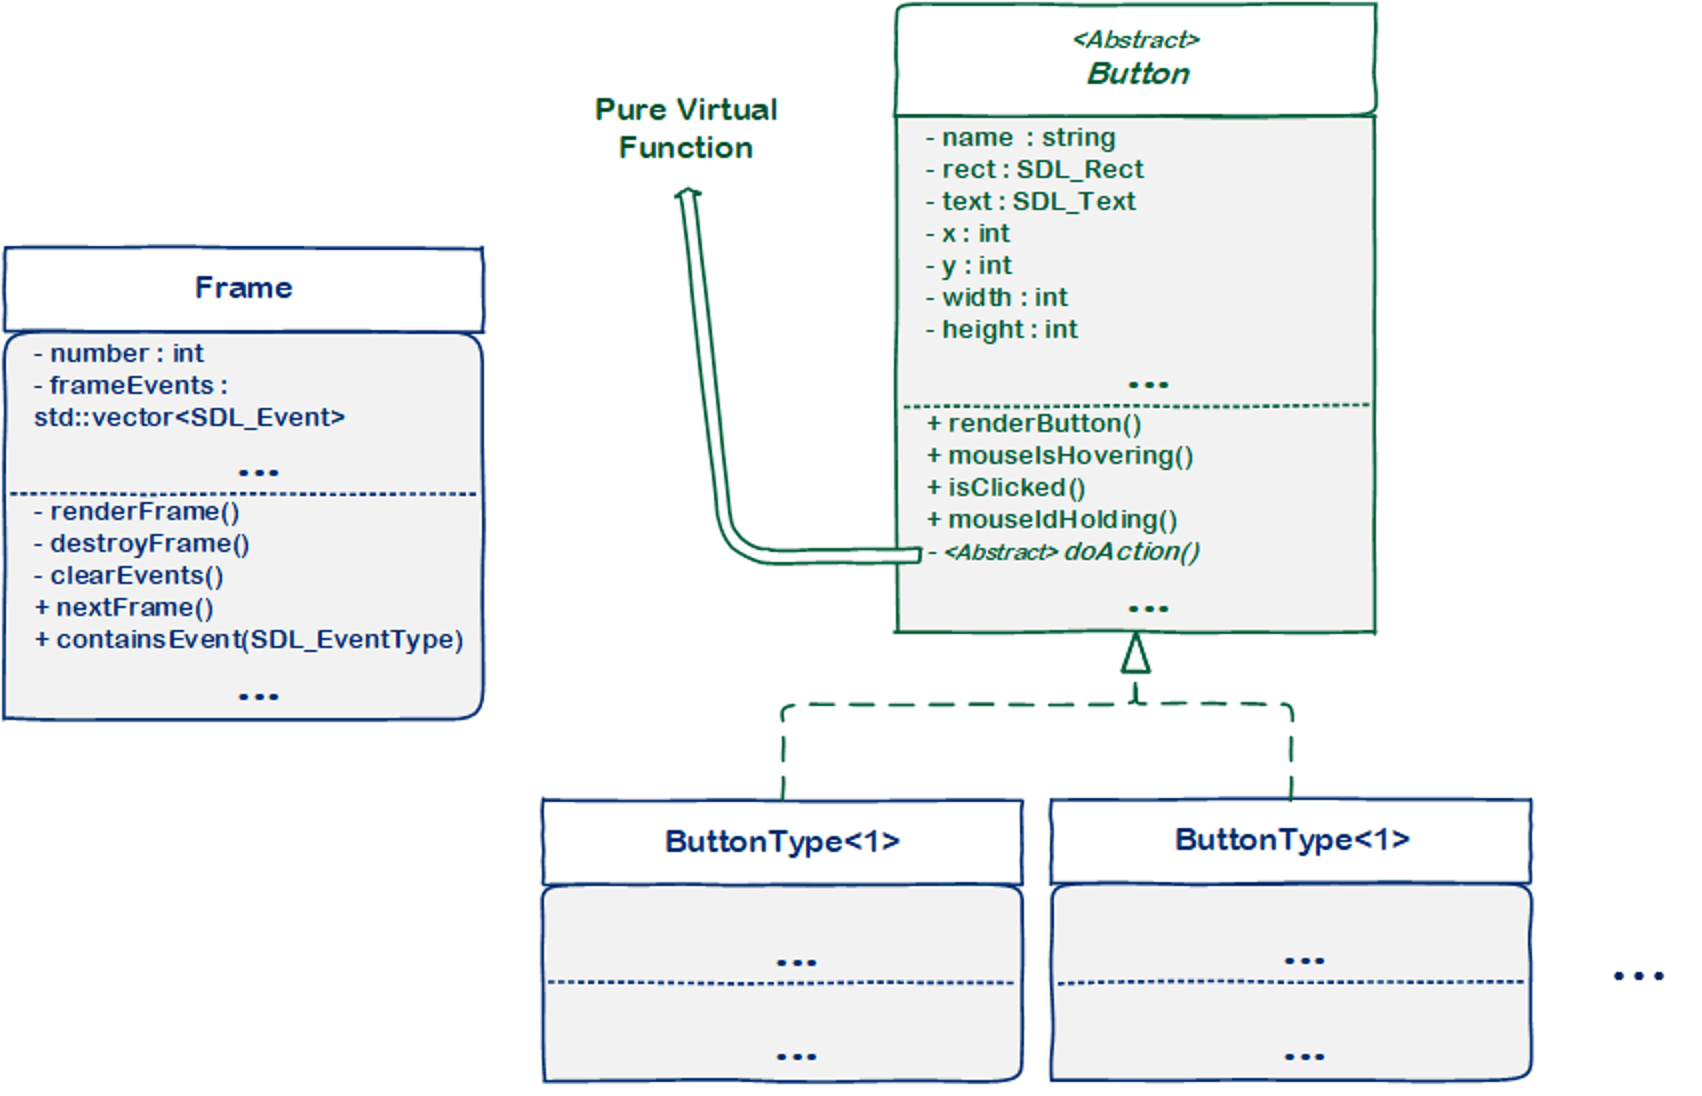
\includegraphics[width=\linewidth,height=.72\textheight,keepaspectratio]{assets/004_p005_02.png}\caption{Diagram or recorded result: Modified nodal analysis.}\label{fig:004_p005_020}\end{figure}
\clearpage
\section{Transient and nonlinear analysis}

Capacitor and inductor companion models depend on the timestep and previous state. Implement the requested transient path, explaining the discretization, initial conditions, and state updates. Backward Euler and trapezoidal integration are discussed in the source. Adaptive steps also change the companion coefficients and may invalidate cached factors. For a diode, use a nonlinear model and Newton linearization rather than assuming every component is a fixed resistor. The worked example uses a 5-V source, 1-kilohm resistance, saturation current 1e-14 A, thermal voltage 0.026 V, ideality factor 1, and an initial voltage of 0.7 V. Its scalar residual is f(V) =\allowbreak{} (5-V)/\allowbreak{}R - I\_\allowbreak{}s(exp(V/\allowbreak{}V\_\allowbreak{}T)-1), with derivative -1/\allowbreak{}R - (I\_\allowbreak{}s/\allowbreak{}V\_\allowbreak{}T)exp(V/\allowbreak{}V\_\allowbreak{}T). Explain convergence tolerance and iteration limits. The RC worked example uses R =\allowbreak{} 1 kilohm, C =\allowbreak{} 1 microfarad, a 5-V step, zero initial voltage, and h =\allowbreak{} 1 microsecond. Backward Euler gives A =\allowbreak{} 1/\allowbreak{}R+\allowbreak{}C/\allowbreak{}h =\allowbreak{} 1.001 S, b =\allowbreak{} 0.005 A, and the first capacitor voltage approximately 0.004995 V. The RLC example uses R =\allowbreak{} 1 kilohm, L =\allowbreak{} 1 millihenry, C =\allowbreak{} 1 microfarad and the same step/\allowbreak{}timestep. Its supplied first-step system is [1,-1;\allowbreak{} -1,-2000] [V;\allowbreak{}I] =\allowbreak{} [0;\allowbreak{}-5], giving approximately 0.00249875 V and 0.00249875 A. The numerical equality of those values depends on the example's coefficients and is not a general physical identity.

\begingroup\small\setlength{\tabcolsep}{3pt}\renewcommand{\arraystretch}{1.18}\begin{longtable}{@{}p{0.3000\linewidth}p{0.3000\linewidth}p{0.3000\linewidth}@{}}
\caption{Transient and nonlinear analysis - numerical data and parameters.}\label{tab:003_p007_table10}\\\toprule
\textbf{Block} & \textbf{Dimensions} & \textbf{Construction} \\ \midrule\endfirsthead \textbf{Block} & \textbf{Dimensions} & \textbf{Construction} \\ \midrule\endhead
G & n x n & Conductance stamps between non-reference nodes \\
B & n x m & Voltage-source incidence \\
C & m x n & B transpose for independent ideal sources \\
D & m x m & Zero for independent ideal voltage sources \\
J & n x 1 & Injected independent source currents \\
E & m x 1 & Independent source voltages \\
\bottomrule\end{longtable}\endgroup
\begin{figure}[!htbp]\centering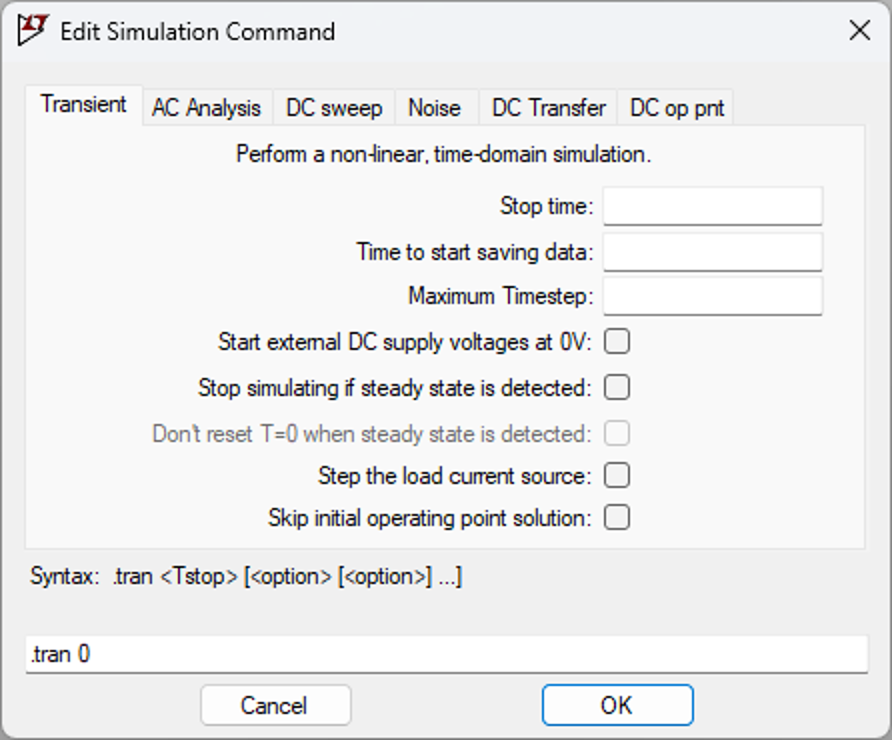
\includegraphics[width=\linewidth,height=.72\textheight,keepaspectratio]{assets/004_p007_01.png}\caption{Diagram or recorded result: Transient and nonlinear analysis.}\label{fig:004_p007_010}\end{figure}
\begin{figure}[!htbp]\centering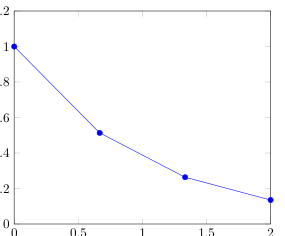
\includegraphics[width=\linewidth,height=.72\textheight,keepaspectratio]{assets/004_p008_vector1.png}\caption{Diagram or recorded result: Transient and nonlinear analysis.}\label{fig:004_p008_vector10}\end{figure}
\begin{figure}[!htbp]\centering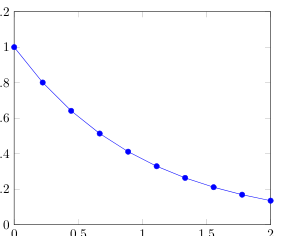
\includegraphics[width=\linewidth,height=.72\textheight,keepaspectratio]{assets/004_p008_vector2.png}\caption{Diagram or recorded result: Transient and nonlinear analysis.}\label{fig:004_p008_vector20}\end{figure}
\begin{figure}[!htbp]\centering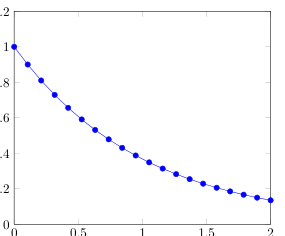
\includegraphics[width=\linewidth,height=.72\textheight,keepaspectratio]{assets/004_p008_vector3.png}\caption{Diagram or recorded result: Transient and nonlinear analysis.}\label{fig:004_p008_vector30}\end{figure}
\clearpage
\section{Component commands and validation}

Support add and delete commands for resistors, capacitors, and inductors. Examples include {\small\ttfamily add R1 VIN GND 2.2k}, {\small\ttfamily add C1 VIN GND 1u}, and {\small\ttfamily add L1 VIN GND 1m}. Identifiers use the corresponding uppercase component prefix. Reject zero or negative passive values, malformed syntax, duplicate names, and deletion of unknown elements. Messages should identify the failed component or argument. Parse bare resistance in ohms and the requested kilo/\allowbreak{}mega prefixes;\allowbreak{} capacitance in farads with micro/\allowbreak{}nano prefixes;\allowbreak{} inductance in henries with milli/\allowbreak{}micro prefixes. Scientific notation such as 2e3 or 1e-6 must be handled consistently. Document case sensitivity so that a prefix cannot silently change a value by orders of magnitude. The optional diode command creates {\small\ttfamily D<name>} between two nodes with the specified D or Z model. Reject unsupported model identifiers and preserve the same duplicate/\allowbreak{}missing-element checks. A diode class alone does not satisfy the nonlinear-analysis requirement.


{\small\ttfamily add GND <node>} establishes the reference and {\small\ttfamily delete GND <node>} removes it according to the prescribed interface. Diagnose a missing node and circuits without a valid reference. {\small\ttfamily nodes} lists node identifiers. {\small\ttfamily list} lists elements, and a component-type filter limits the output. {\small\ttfamily rename node <old> <new>} must reject collisions and missing originals and update every connected endpoint reference.

\begin{figure}[!htbp]\centering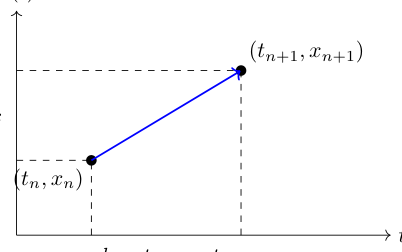
\includegraphics[width=\linewidth,height=.72\textheight,keepaspectratio]{assets/003_p011_vector1.png}\caption{Diagram or recorded result: Component commands and validation.}\label{fig:003_p011_vector10}\end{figure}
\begin{figure}[!htbp]\centering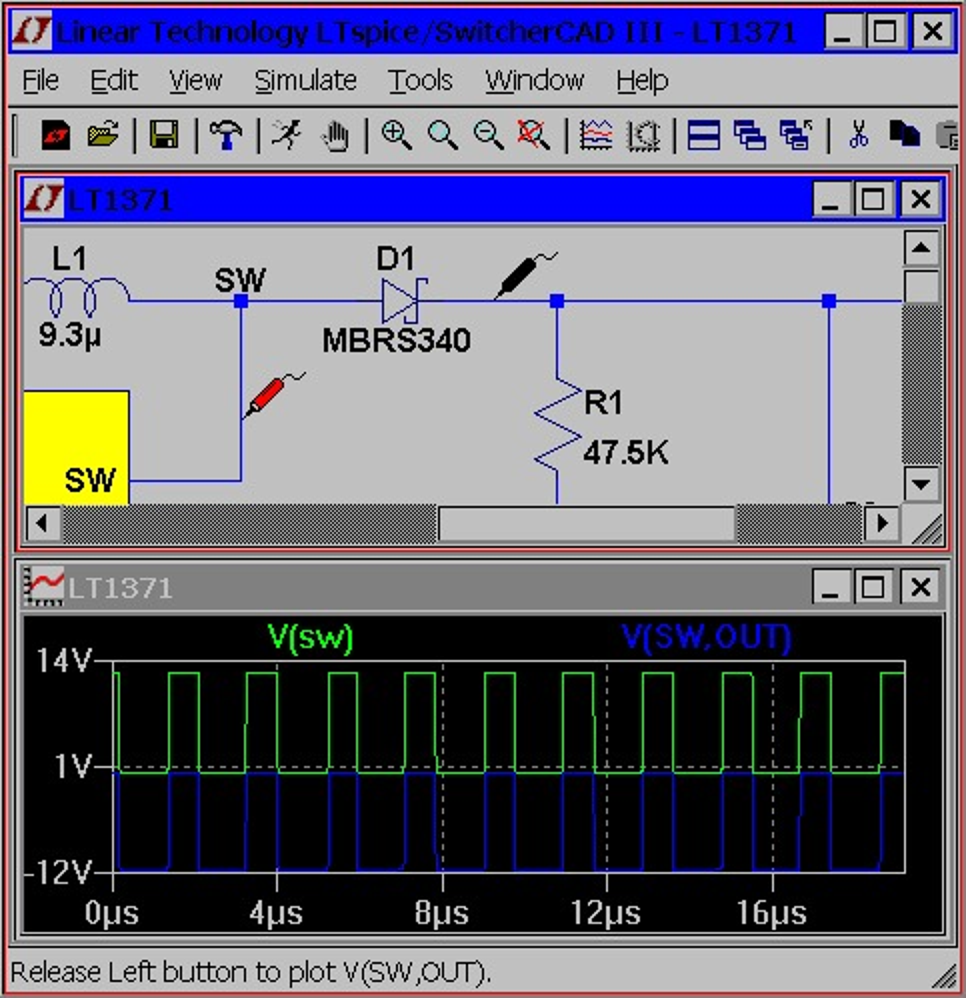
\includegraphics[width=\linewidth,height=.72\textheight,keepaspectratio]{assets/004_p009_01.png}\caption{Diagram or recorded result: Component commands and validation.}\label{fig:004_p009_010}\end{figure}
\begin{figure}[!htbp]\centering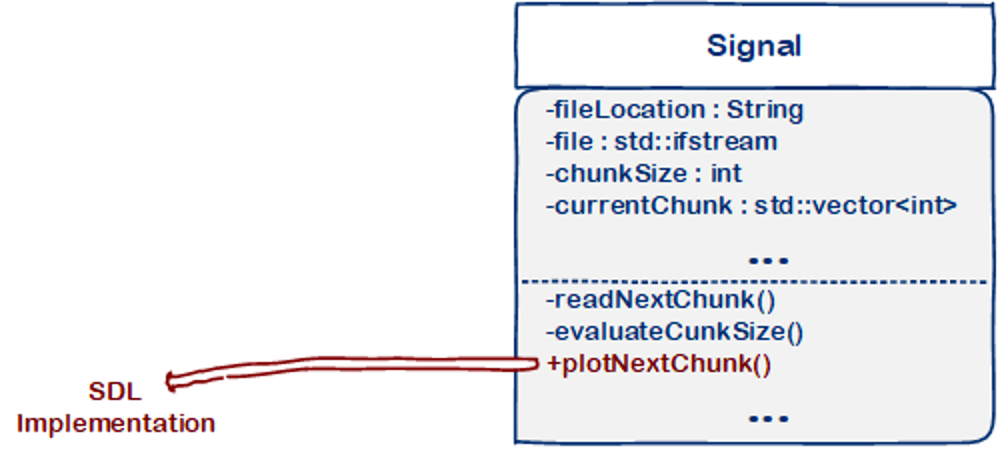
\includegraphics[width=\linewidth,height=.72\textheight,keepaspectratio]{assets/004_p010_01.png}\caption{Diagram or recorded result: Component commands and validation.}\label{fig:004_p010_010}\end{figure}
\begin{figure}[!htbp]\centering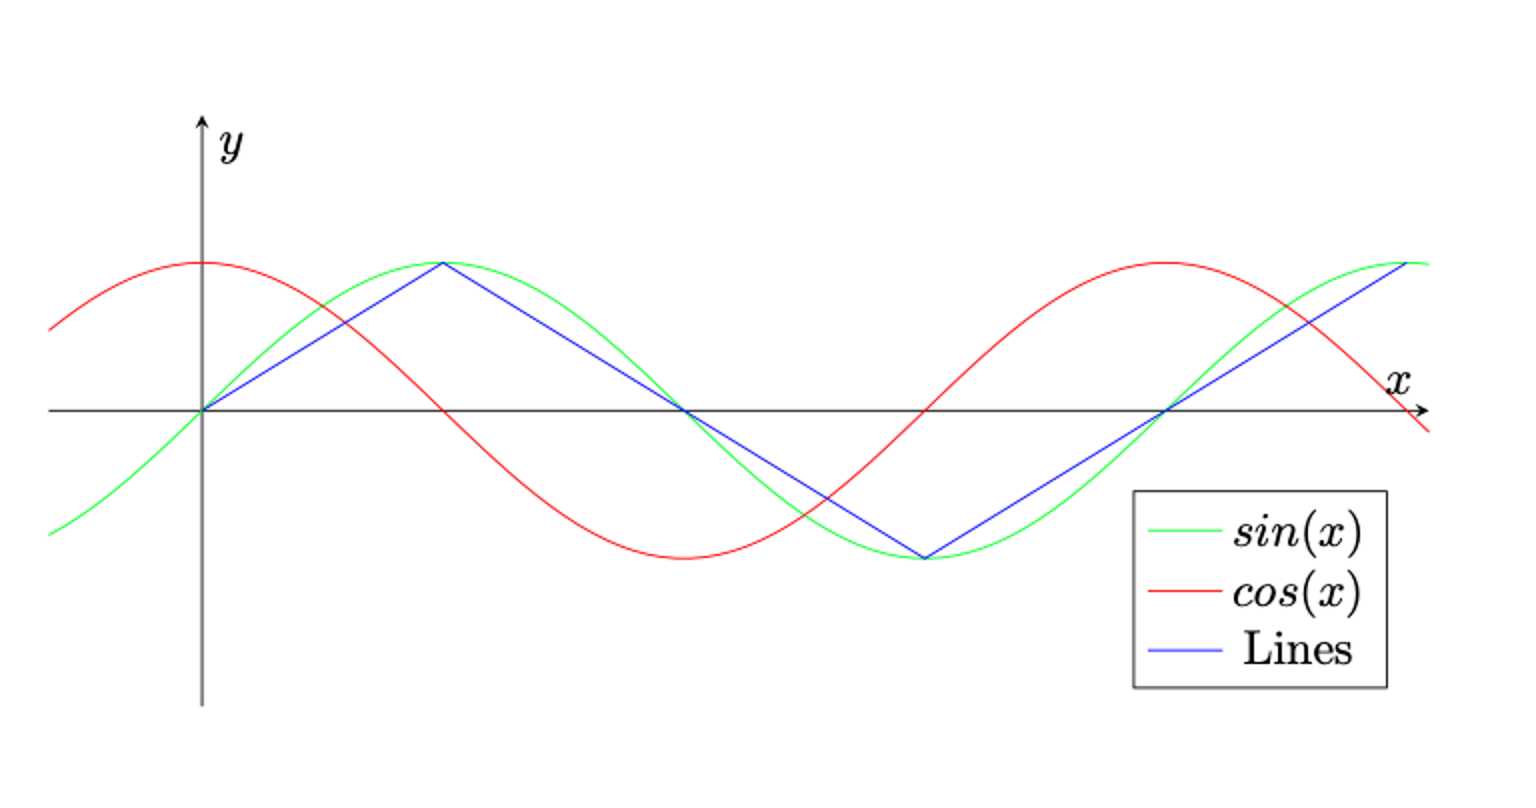
\includegraphics[width=\linewidth,height=.72\textheight,keepaspectratio]{assets/004_p011_01.png}\caption{Diagram or recorded result: Component commands and validation.}\label{fig:004_p011_010}\end{figure}
\clearpage
\section{Sources and output requests}

Create independent voltage and current sources with names, endpoints, and values. Sinusoidal voltage-source syntax includes offset, amplitude, and frequency. The optional PULSE source includes initial/\allowbreak{}final values, delay, rise/\allowbreak{}fall times, width, and period;\allowbreak{} state the accepted punctuation and units explicitly. Controlled-source types are E for voltage-controlled voltage source, G for voltage-controlled current source, H for current-controlled voltage source, and F for current-controlled current source. Voltage-controlled devices refer to control endpoints;\allowbreak{} current-controlled devices refer to a named control source. Validate those references before assembling equations. Transient requests include TRAN with timestep, stop time, and the specified optional start/\allowbreak{}max-step parameters. Requested output variables can include V(node) and I(element), with more than one variable in a print request. Optional DC sweeping specifies a source, start, stop, increment, and requested outputs. Define consistent sampling and column order. Missing analysis parameters, invalid timesteps, unknown variables, or undefined controls are errors rather than empty successful results.

\begin{figure}[!htbp]\centering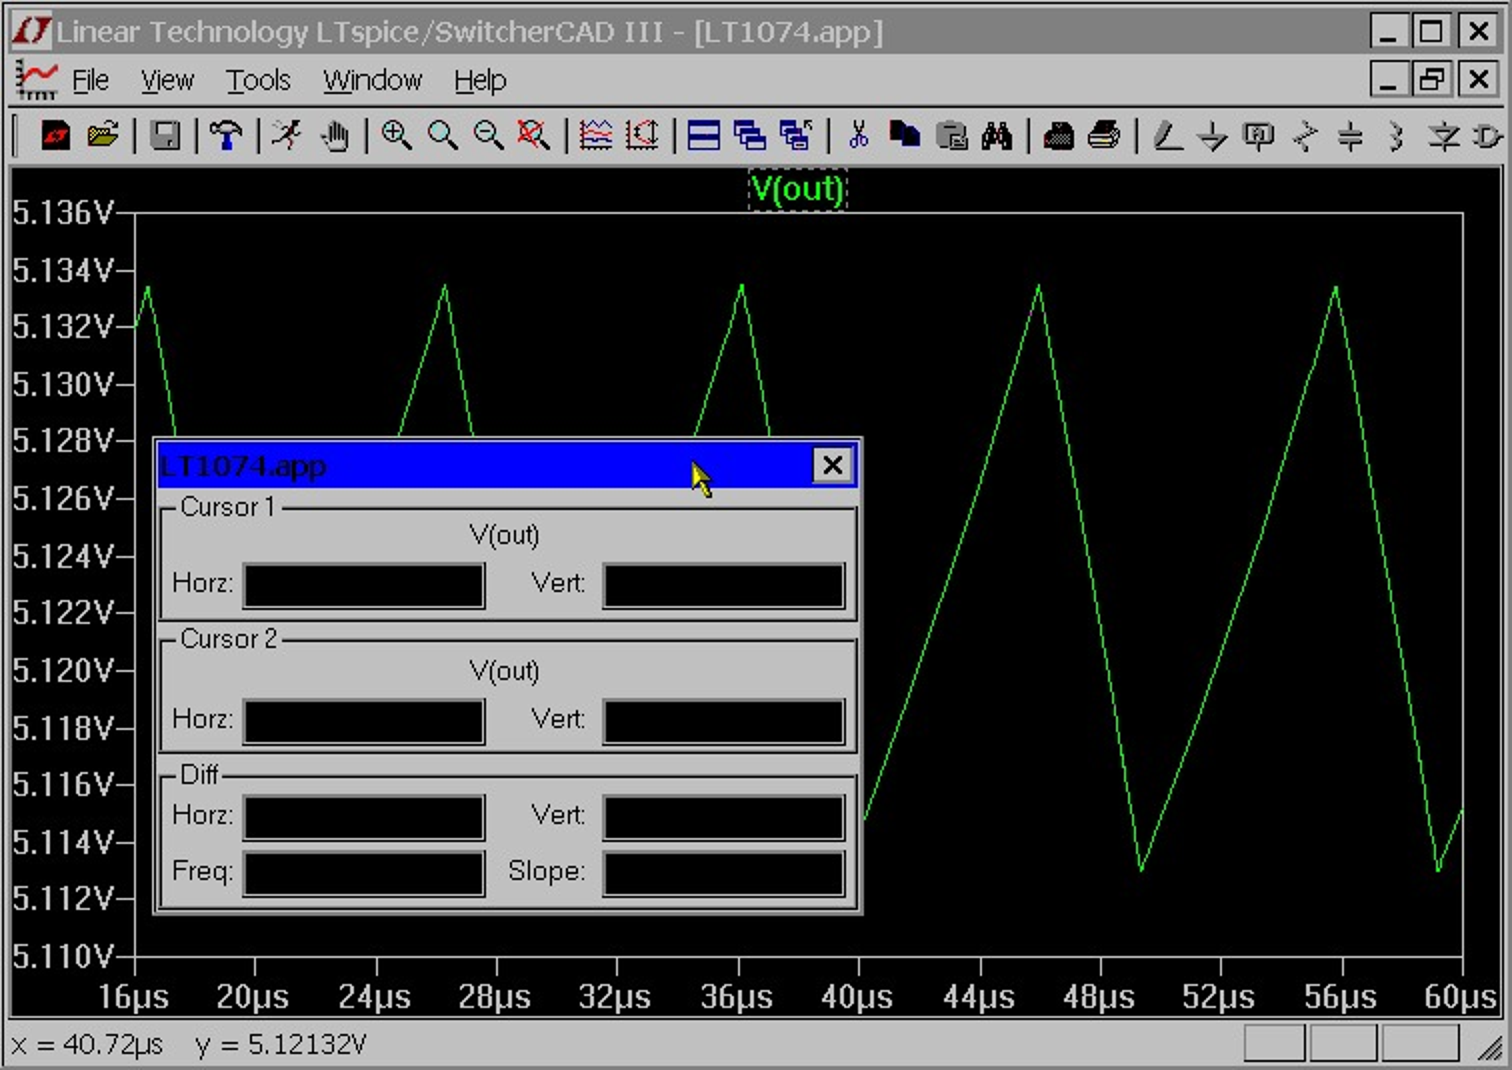
\includegraphics[width=\linewidth,height=.72\textheight,keepaspectratio]{assets/004_p014_01.png}\caption{Diagram or recorded result: Sources and output requests.}\label{fig:004_p014_010}\end{figure}
\clearpage
\section{Netlists, files, and console workflow}

Support the assignment's netlist representation as well as interactive commands. The simple divider example describes a 5-V source and 1000/\allowbreak{}2000-ohm series resistors. The supplied more advanced example includes a sinusoidal source, resistor, capacitor, transient/\allowbreak{}AC directives, and an end marker. Present the existing schematic files in a selection menu. Invalid selection produces the prescribed error and returns to a usable state. {\small\ttfamily NewFile <file\_\allowbreak{}path>} creates a new file through the documented workflow. File parsing, interactive input, and graphical extensions should share the same validated circuit model.

\begin{figure}[!htbp]\centering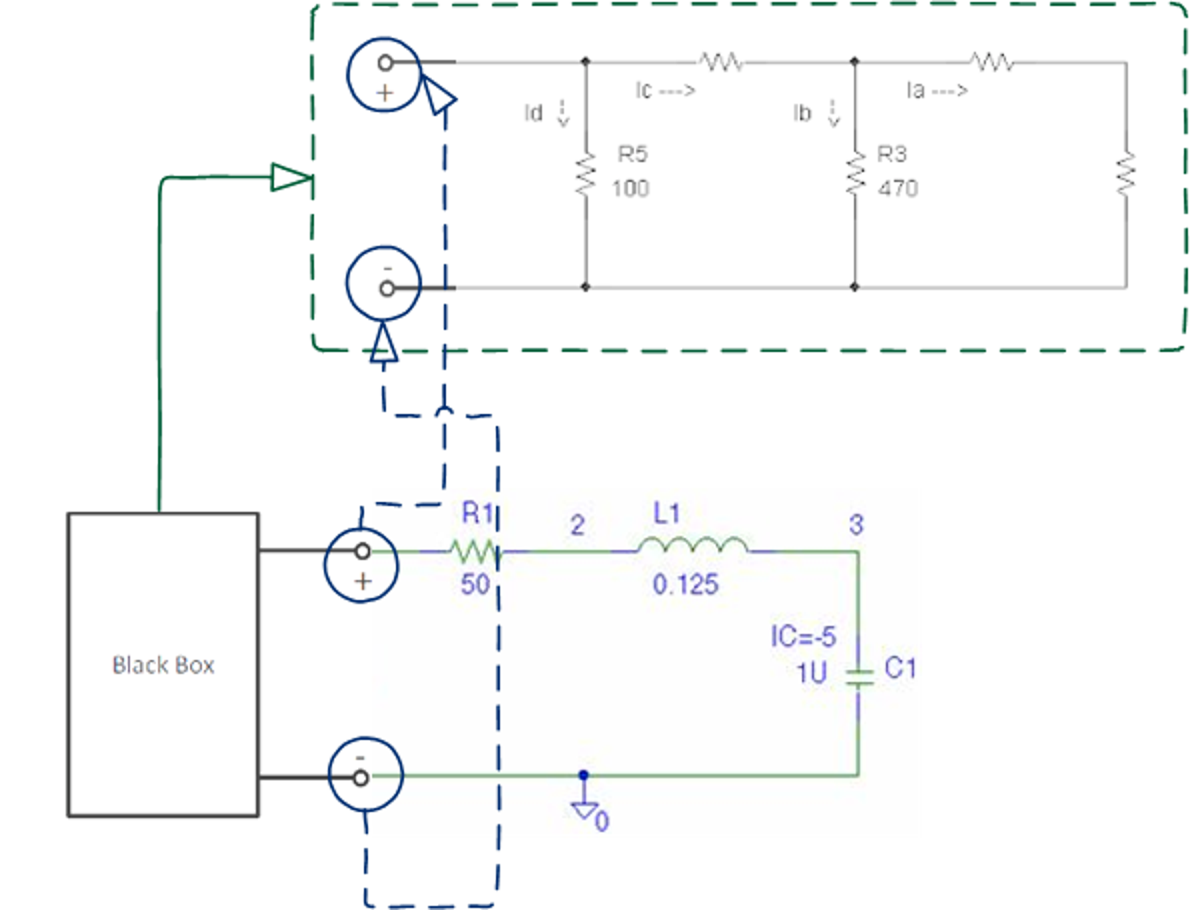
\includegraphics[width=\linewidth,height=.72\textheight,keepaspectratio]{assets/004_p015_01.png}\caption{Diagram or recorded result: Netlists, files, and console workflow.}\label{fig:004_p015_010}\end{figure}
\clearpage
\section{Required error handling and deliverables}

Diagnose missing ground, floating nodes/\allowbreak{}subcircuits, contradictory ideal-source constraints, nonpositive passive values, undefined controls, duplicate identifiers, malformed commands, and missing simulation parameters. A disconnected drawing is not necessarily invalid if each electrical subcircuit has a valid reference;\allowbreak{} explain the actual rank/\allowbreak{}connectivity issue. Submit the C+\allowbreak{}+\allowbreak{} implementation and the requested results with readable object-oriented structure. The mandatory transient implementation and optional features must remain distinguishable.


\section{Circuit simulator implementation assignment: graphical interface and persistence}
\begin{figure}[!htbp]\centering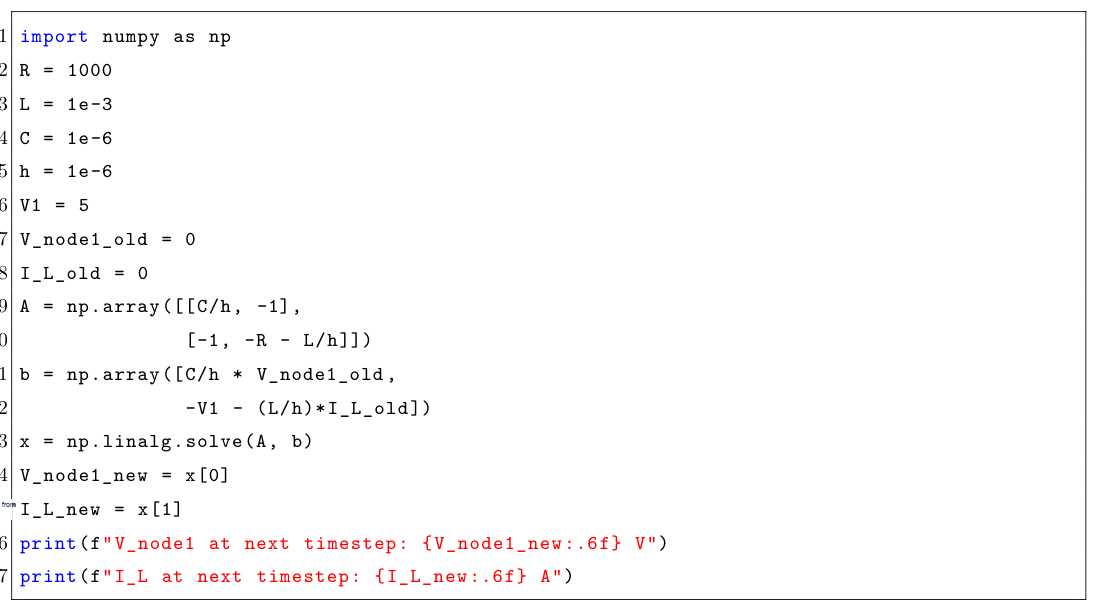
\includegraphics[width=\linewidth,height=.72\textheight,keepaspectratio]{assets/003_p018_vector1.png}\caption{Implementation and output: Required error handling and deliverables.}\label{fig:003_p018_vector10}\end{figure}
\begin{figure}[!htbp]\centering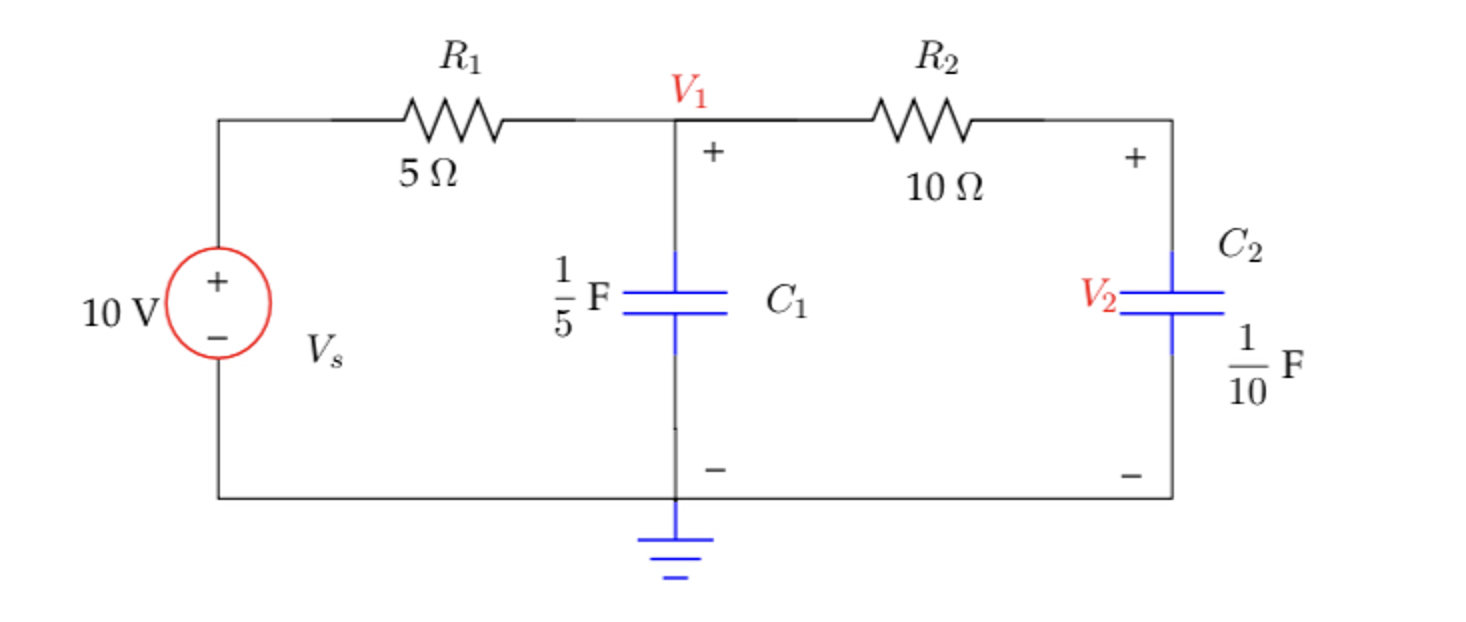
\includegraphics[width=\linewidth,height=.72\textheight,keepaspectratio]{assets/004_p017_01.png}\caption{Diagram or recorded result: Required error handling and deliverables.}\label{fig:004_p017_010}\end{figure}
\begin{figure}[!htbp]\centering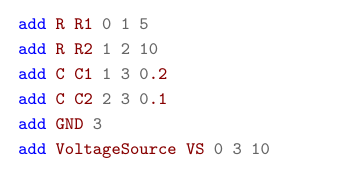
\includegraphics[width=\linewidth,height=.72\textheight,keepaspectratio]{assets/004_p017_vector1.png}\caption{Diagram or recorded result: Required error handling and deliverables.}\label{fig:004_p017_vector10}\end{figure}
\begin{figure}[!htbp]\centering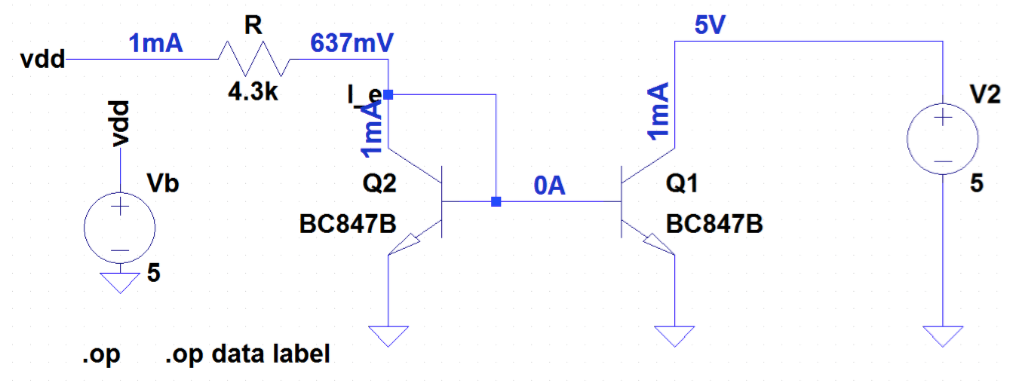
\includegraphics[width=\linewidth,height=.72\textheight,keepaspectratio]{assets/004_p018_01.png}\caption{Diagram or recorded result: Required error handling and deliverables.}\label{fig:004_p018_010}\end{figure}
\begingroup\small\setlength{\tabcolsep}{3pt}\renewcommand{\arraystretch}{1.18}\begin{longtable}{@{}p{0.3000\linewidth}p{0.3000\linewidth}p{0.3000\linewidth}@{}}
\caption{Required error handling and deliverables - numerical data and parameters.}\label{tab:004_p019_table10}\\\toprule
\textbf{Symbol} & \textbf{Meaning} & \textbf{Unit} \\ \midrule\endfirsthead \textbf{Symbol} & \textbf{Meaning} & \textbf{Unit} \\ \midrule\endhead
omega\_\allowbreak{}start & Lower angular-frequency bound & rad/\allowbreak{}s \\
omega\_\allowbreak{}stop & Upper angular-frequency bound & rad/\allowbreak{}s \\
N & Number of steps & dimensionless \\
\bottomrule\end{longtable}\endgroup
\begingroup\small\setlength{\tabcolsep}{3pt}\renewcommand{\arraystretch}{1.18}\begin{longtable}{@{}p{0.3000\linewidth}p{0.3000\linewidth}p{0.3000\linewidth}@{}}
\caption{Required error handling and deliverables - numerical data and parameters.}\label{tab:004_p019_table20}\\\toprule
\textbf{Symbol} & \textbf{Meaning} & \textbf{Unit} \\ \midrule\endfirsthead \textbf{Symbol} & \textbf{Meaning} & \textbf{Unit} \\ \midrule\endhead
phi\_\allowbreak{}start & Lower phase bound & rad \\
phi\_\allowbreak{}stop & Upper phase bound & rad \\
omega\_\allowbreak{}base & Base angular frequency & rad/\allowbreak{}s \\
N & Number of steps & dimensionless \\
\bottomrule\end{longtable}\endgroup
\clearpage
\section{Scope, feature status, and graphical framework}

Extend the numerical/\allowbreak{}console engine with an object-oriented SDL2 graphical interface. The assignment uses colored boxes:\allowbreak{} red-box features are bonus work for two-person teams and mandatory for three-person teams;\allowbreak{} purple-box features are bonus work for three-person teams;\allowbreak{} yellow boxes provide guidance. Use an event loop, window/\allowbreak{}renderer abstractions, and a reasonable frame rate. Handle input and redraw without blocking the interface with long numerical work. The assignment points to SDL resources and examples;\allowbreak{} document the development libraries and assets required by the chosen build.

\begingroup\small\setlength{\tabcolsep}{3pt}\renewcommand{\arraystretch}{1.18}\begin{longtable}{@{}p{0.3000\linewidth}p{0.3000\linewidth}p{0.3000\linewidth}@{}}
\caption{Scope, feature status, and graphical framework - numerical data and parameters.}\label{tab:003_p019_table10}\\\toprule
\textbf{Problem} & \textbf{Equation} & \textbf{Numerical approach} \\ \midrule\endfirsthead \textbf{Problem} & \textbf{Equation} & \textbf{Numerical approach} \\ \midrule\endhead
Linear algebraic & A x =\allowbreak{} b & Pivoted LU or sparse direct solver \\
First-order differential & dy/\allowbreak{}dt =\allowbreak{} f(t,y) & Backward Euler or trapezoidal integration \\
Nonlinear & f(x) =\allowbreak{} 0 & Newton-Raphson \\
\bottomrule\end{longtable}\endgroup
\begin{figure}[!htbp]\centering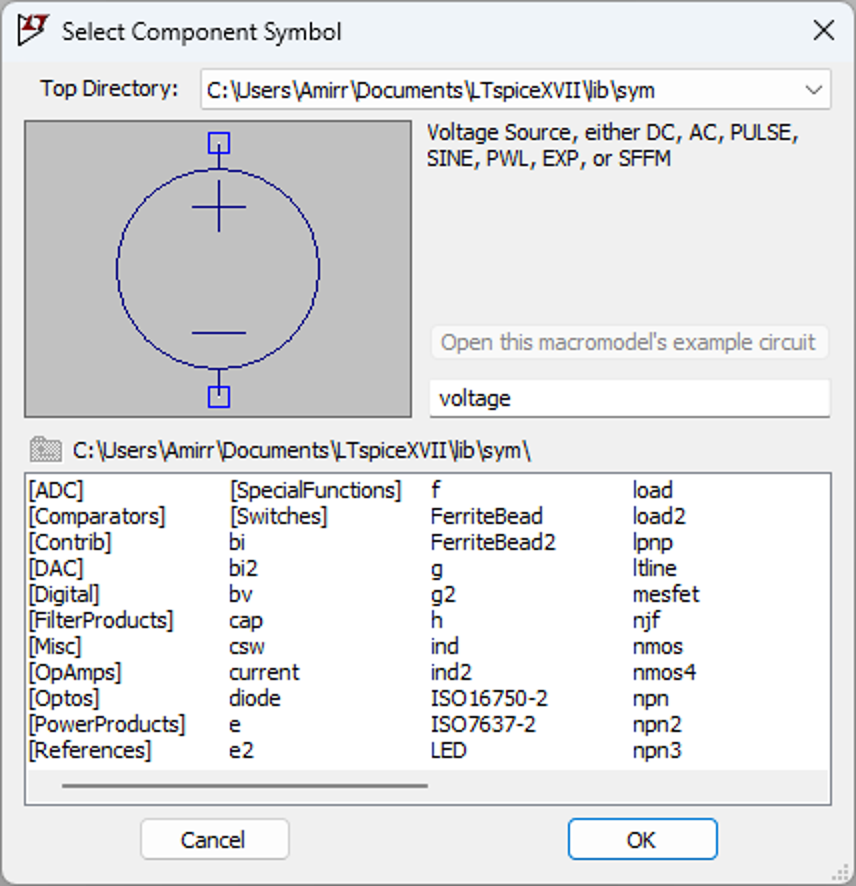
\includegraphics[width=\linewidth,height=.72\textheight,keepaspectratio]{assets/004_p021_01.png}\caption{Diagram or recorded result: Scope, feature status, and graphical framework.}\label{fig:004_p021_010}\end{figure}
\clearpage
\section{Signal data and plotted results}

A Signal or WaveformSource object holds a sampled array and timing information such as duration and sample rate. The example signal exp(-t)u(t) on 0 to 2 seconds illustrates sampling at 2, 5, and 10 samples per second. Connecting sample points for display does not increase the numerical simulation's accuracy. Expose stop time, saved-output start time, and maximum step through the simulation interface. Voltage probes select nodes relative to ground;\allowbreak{} current and power probes select appropriate components and sign conventions. A 10-second trace sampled at 10 kHz contains 100,000 values per scalar channel. Discuss whole-array loading versus chunked processing and memory usage. Support multiple traces with different colors, legends, renaming, and color selection. Existing traces should keep stable colors when another trace is added. Evaluate expressions such as K*(V(R1+\allowbreak{})-V(R1-)) through a defined expression parser or operator interface. Distinguish a computed sum of component signals from sequentially drawing unrelated traces. Provide horizontal/\allowbreak{}vertical grids, scale controls, and auto-fit with appropriate padding. A single cursor reports a selected coordinate/\allowbreak{}value. Two cursors report horizontal/\allowbreak{}vertical differences and slope where meaningful. Frequency measurement is not required by the stated cursor task. Preserve the original signal UML and plot examples.

\begin{figure}[!htbp]\centering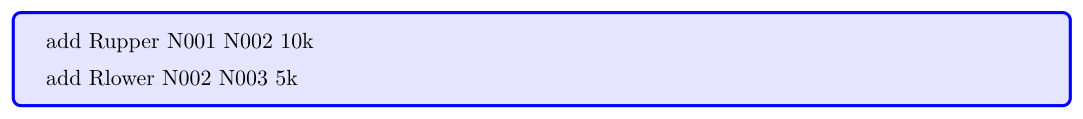
\includegraphics[width=\linewidth,height=.72\textheight,keepaspectratio]{assets/003_p022_vector2.png}\caption{Diagram or recorded result: Signal data and plotted results.}\label{fig:003_p022_vector20}\end{figure}
\begingroup\small\setlength{\tabcolsep}{3pt}\renewcommand{\arraystretch}{1.18}\begin{longtable}{@{}p{0.1400\linewidth}p{0.1400\linewidth}p{0.1400\linewidth}p{0.1400\linewidth}p{0.1400\linewidth}p{0.1400\linewidth}@{}}
\caption{Signal data and plotted results - numerical data and parameters.}\label{tab:004_p023_table10}\\\toprule
\textbf{Address} & \textbf{0x0000} & \textbf{0x0001} & \textbf{0x0002} & \textbf{0x0003} & \textbf{...} \\ \midrule\endfirsthead \textbf{Address} & \textbf{0x0000} & \textbf{0x0001} & \textbf{0x0002} & \textbf{0x0003} & \textbf{...} \\ \midrule\endhead
Value & 0xab & 0xcd & 0xef & 0xa2 & ... \\
\bottomrule\end{longtable}\endgroup
\begin{figure}[!htbp]\centering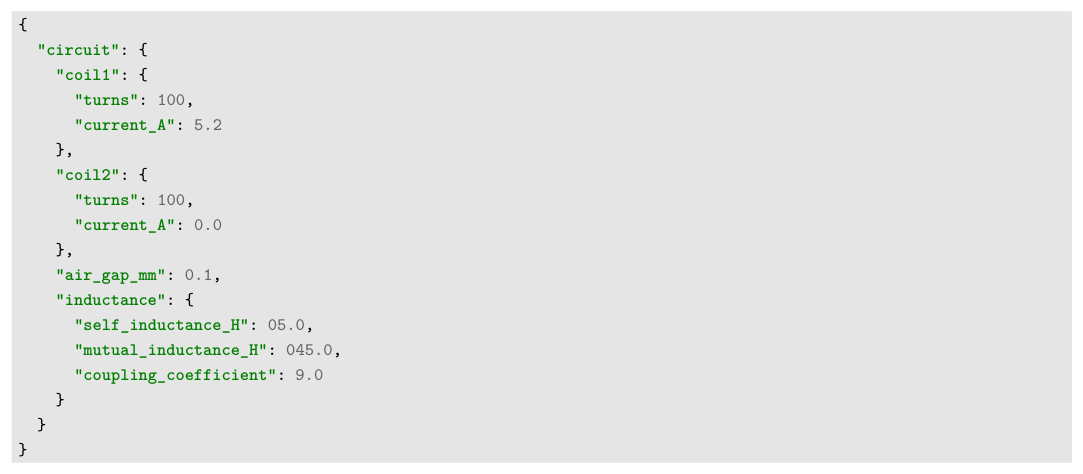
\includegraphics[width=\linewidth,height=.72\textheight,keepaspectratio]{assets/004_p023_vector1.png}\caption{Diagram or recorded result: Signal data and plotted results.}\label{fig:004_p023_vector10}\end{figure}
\clearpage
\section{Subcircuits, schematic drawing, and node labels}

Allow users to select a two-terminal one-port subcircuit, save it, and reuse it as a black-box component with two visible terminals. Its internal ground/\allowbreak{}reference policy must be explicit. A graphical rectangle can represent the saved subcircuit. The optional Thevenin/\allowbreak{}Norton reduction is restricted by the assignment to suitable linear resistive circuits;\allowbreak{} arbitrary nonlinear or dynamic circuits cannot be replaced by a constant source/\allowbreak{}resistance pair. Draw components, values, nodes, and connecting wires. Maintain a distinction between graphical position and electrical connectivity. Support the required placement, zoom/\allowbreak{}pan, and connection workflows. Labels with the same node name denote the same electrical node even when the drawing does not contain a visible wire between them. Multiple elements between the same pair of nodes must remain independently identifiable.

\begin{figure}[!htbp]\centering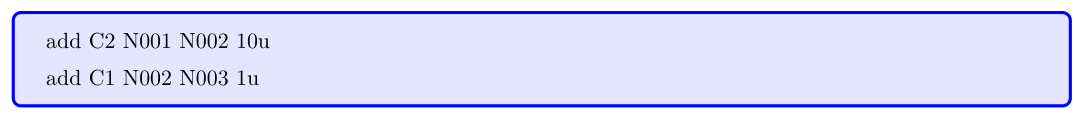
\includegraphics[width=\linewidth,height=.72\textheight,keepaspectratio]{assets/003_p024_vector3.png}\caption{Diagram or recorded result: Subcircuits, schematic drawing, and node labels.}\label{fig:003_p024_vector30}\end{figure}
\begin{figure}[!htbp]\centering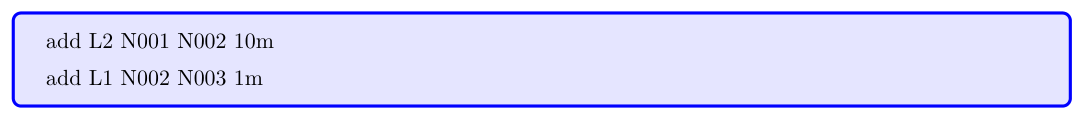
\includegraphics[width=\linewidth,height=.72\textheight,keepaspectratio]{assets/003_p026_vector4.png}\caption{Diagram or recorded result: Subcircuits, schematic drawing, and node labels.}\label{fig:003_p026_vector40}\end{figure}
\begin{figure}[!htbp]\centering
\includegraphics[width=\linewidth,height=.72\textheight,keepaspectratio]{assets/004_p025_01.png}\caption{Diagram or recorded result: Subcircuits, schematic drawing, and node labels.}\label{fig:004_p025_010}\end{figure}
\begin{figure}[!htbp]\centering
\includegraphics[width=\linewidth,height=.72\textheight,keepaspectratio]{assets/004_p025_02.png}\caption{Diagram or recorded result: Subcircuits, schematic drawing, and node labels.}\label{fig:004_p025_020}\end{figure}
\begin{figure}[!htbp]\centering
\includegraphics[width=\linewidth,height=.72\textheight,keepaspectratio]{assets/004_p025_vector1.png}\caption{Diagram or recorded result: Subcircuits, schematic drawing, and node labels.}\label{fig:004_p025_vector10}\end{figure}
\begin{figure}[!htbp]\centering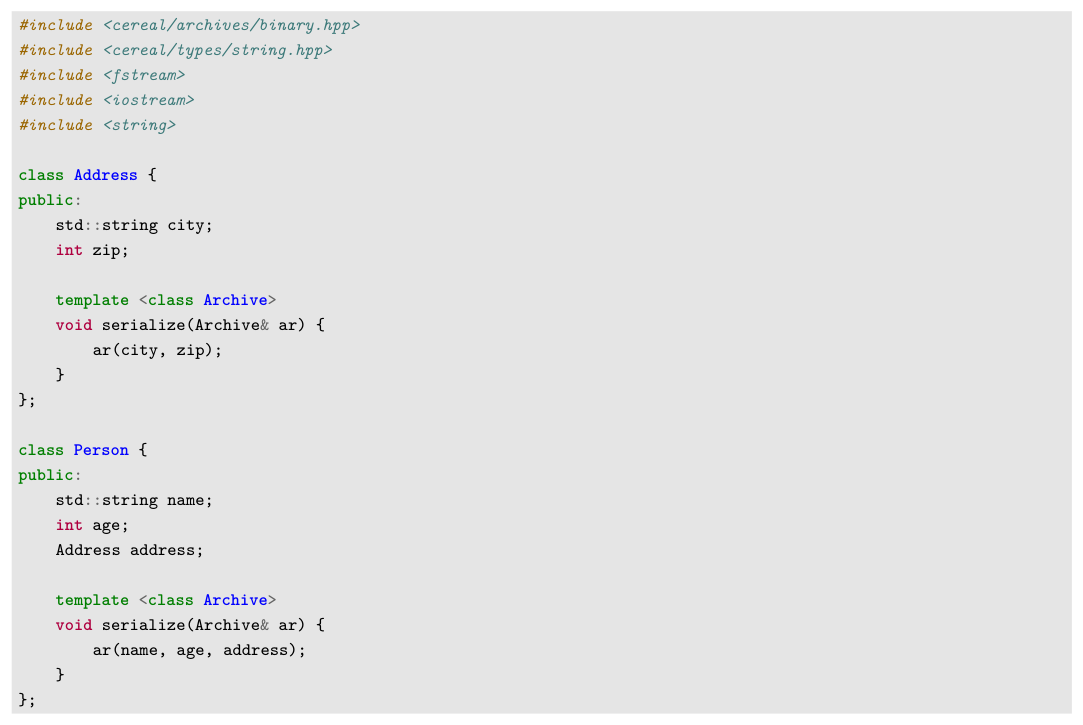
\includegraphics[width=\linewidth,height=.72\textheight,keepaspectratio]{assets/004_p027_vector1.png}\caption{Implementation and output: Subcircuits, schematic drawing, and node labels.}\label{fig:004_p027_vector10}\end{figure}
\clearpage
\section{AC and phase sweep controls}

AC analysis uses a sinusoidal source and a frequency range with a specified number of points. The interface offers octave, decade, and linear spacing with start/\allowbreak{}stop frequency. Clearly state whether input is frequency in hertz or angular frequency in radians per second;\allowbreak{} the assignment's omega notation must not silently be interpreted as hertz. The phase-sweep interface sets base frequency, start/\allowbreak{}stop phase, and point count. Sweeping the phase of a single source in an otherwise linear time-invariant circuit does not change the magnitude of its transfer response;\allowbreak{} it shifts phase. Distinguish this input-phase experiment from plotting the transfer function's phase versus frequency. The transient menu includes stop time, saved-output start time, and maximum step. The Node Library makes all implemented phase-1 element types available for graphical placement and also exposes user-defined subcircuits. The File menu lists existing schematics and permits selection. A separate Library menu loads saved subcircuits from a library folder. The Scope menu controls result plots and the display features described above.

\begin{figure}[!htbp]\centering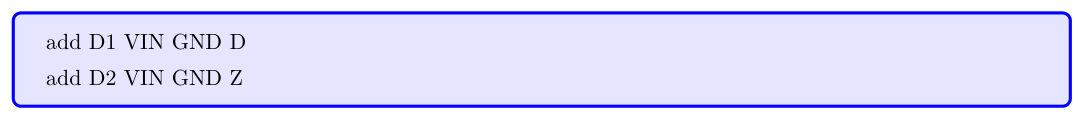
\includegraphics[width=\linewidth,height=.72\textheight,keepaspectratio]{assets/003_p027_vector5.png}\caption{Diagram or recorded result: AC and phase sweep controls.}\label{fig:003_p027_vector50}\end{figure}
\begin{figure}[!htbp]\centering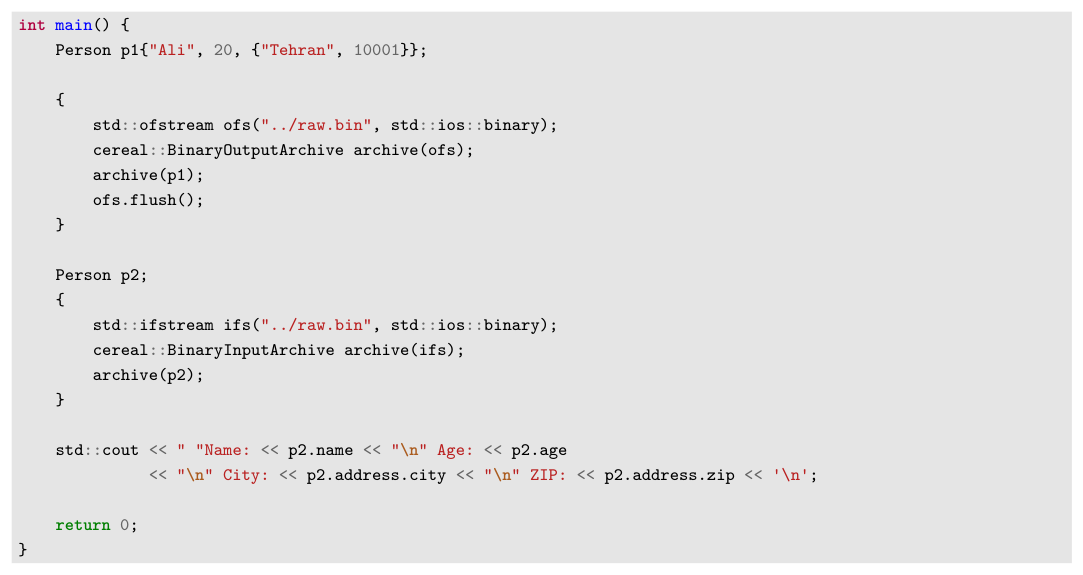
\includegraphics[width=\linewidth,height=.72\textheight,keepaspectratio]{assets/004_p028_vector1.png}\caption{Diagram or recorded result: AC and phase sweep controls.}\label{fig:004_p028_vector10}\end{figure}
\begin{figure}[!htbp]\centering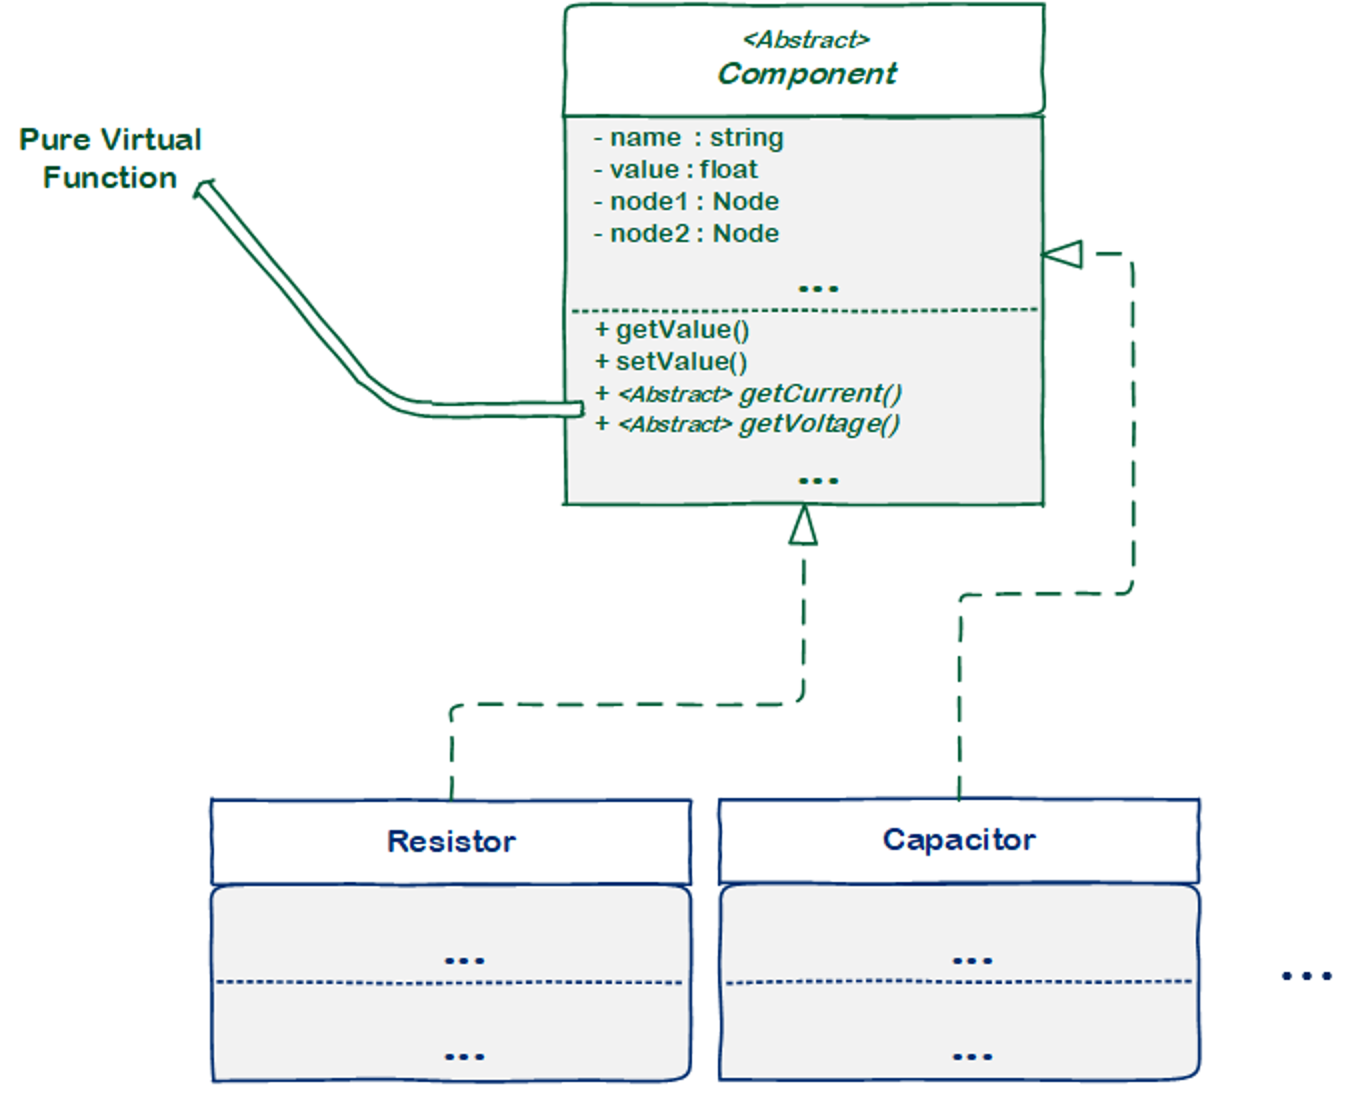
\includegraphics[width=\linewidth,height=.72\textheight,keepaspectratio]{assets/004_p029_01.png}\caption{Diagram or recorded result: AC and phase sweep controls.}\label{fig:004_p029_010}\end{figure}
\begin{figure}[!htbp]\centering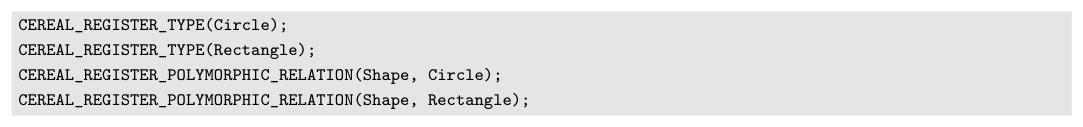
\includegraphics[width=\linewidth,height=.72\textheight,keepaspectratio]{assets/004_p029_vector1.png}\caption{Diagram or recorded result: AC and phase sweep controls.}\label{fig:004_p029_vector10}\end{figure}
\begin{figure}[!htbp]\centering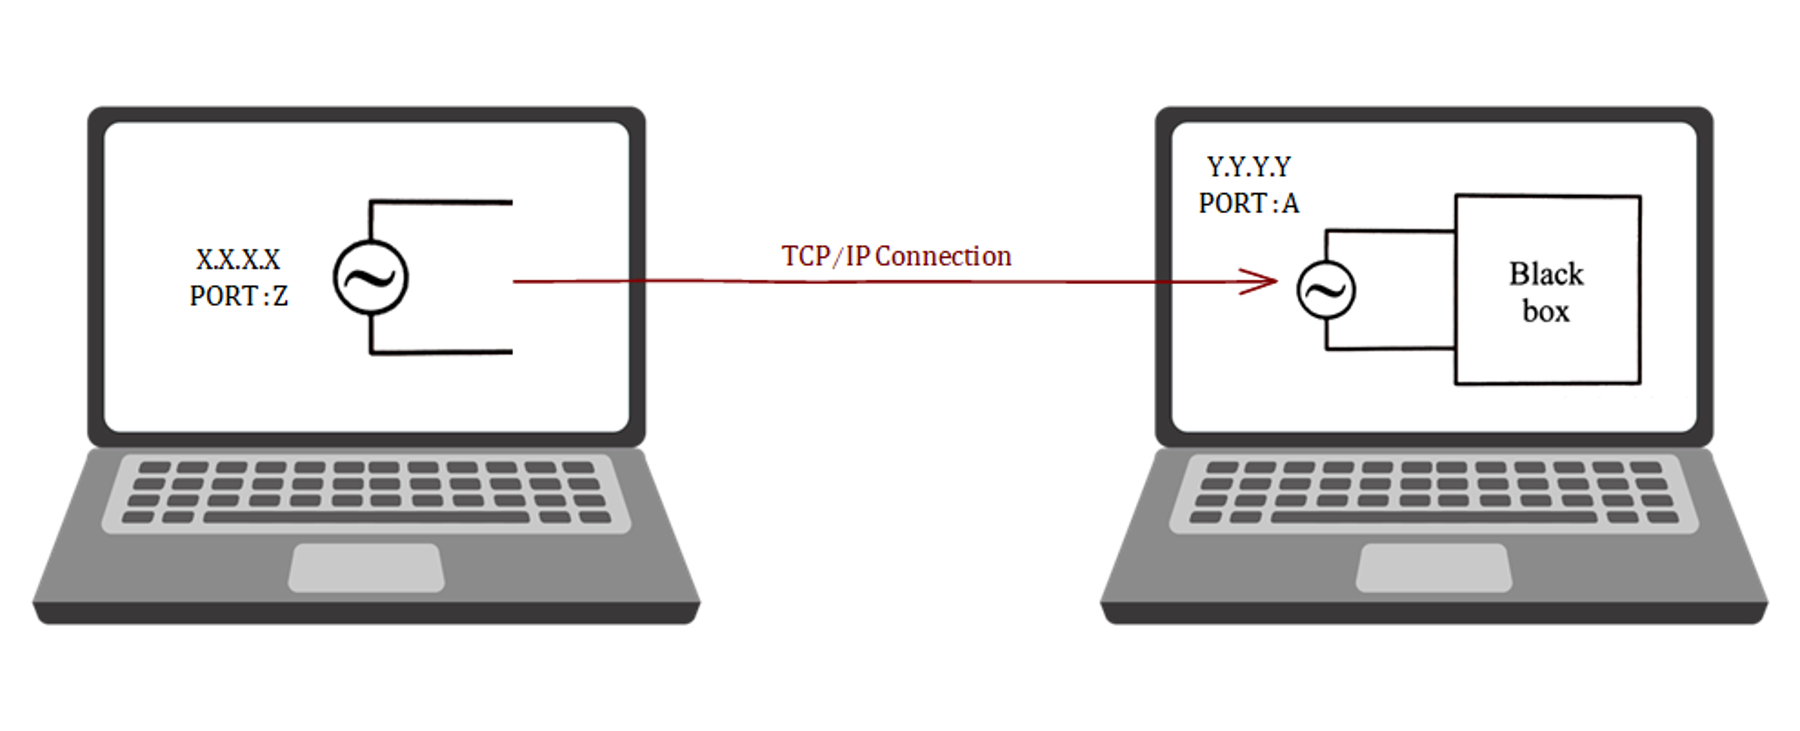
\includegraphics[width=\linewidth,height=.72\textheight,keepaspectratio]{assets/004_p030_01.png}\caption{Diagram or recorded result: AC and phase sweep controls.}\label{fig:004_p030_010}\end{figure}
\begin{figure}[!htbp]\centering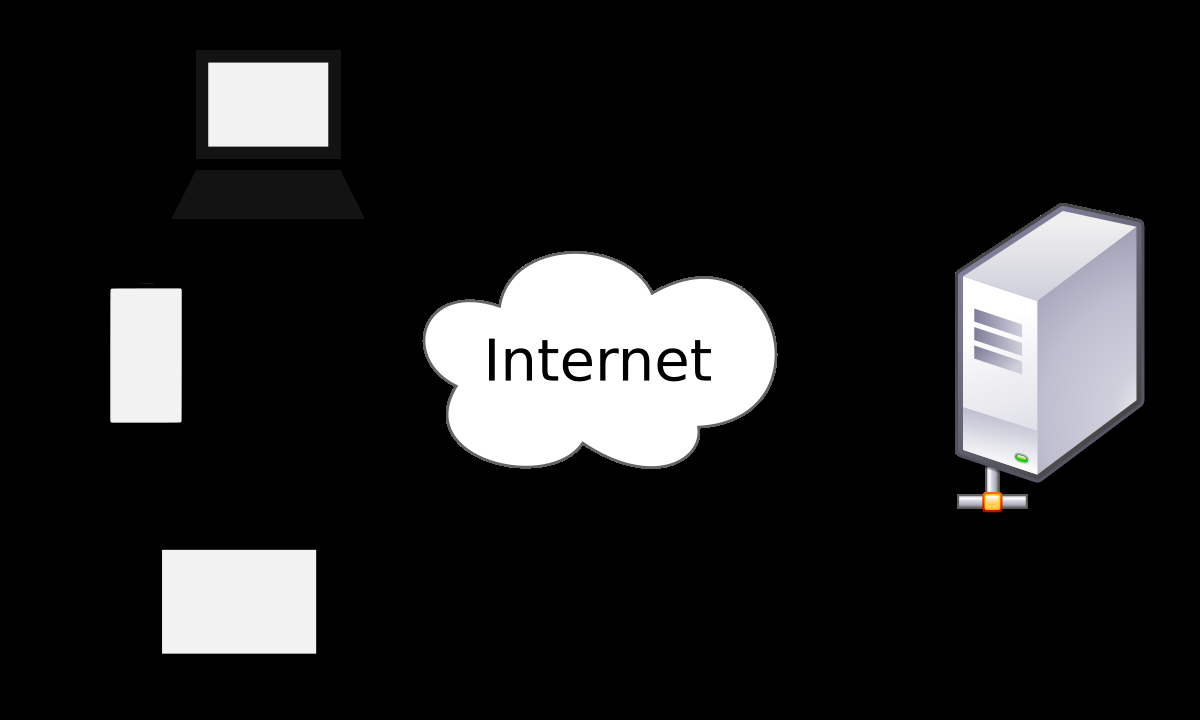
\includegraphics[width=\linewidth,height=.72\textheight,keepaspectratio]{assets/004_p030_02.png}\caption{Diagram or recorded result: AC and phase sweep controls.}\label{fig:004_p030_020}\end{figure}
\clearpage
\section{Project storage requirements}

Save the graphical schematic, numerical circuit description, analysis settings, output signals, and user-defined subcircuits. A project folder should contain enough information to reconstruct both the drawing and the electrical analysis without manually re-entering values. Store reusable subcircuits separately in the library. Define which values are authoritative so that graphical labels and the numerical model do not diverge after loading. The source emphasizes convenient object serialization over elaborate low-level storage optimization. A generic database/\allowbreak{}storage class can provide save and load operations, but each object still needs a well-defined representation, versioning, and reference reconstruction.

\begin{figure}[!htbp]\centering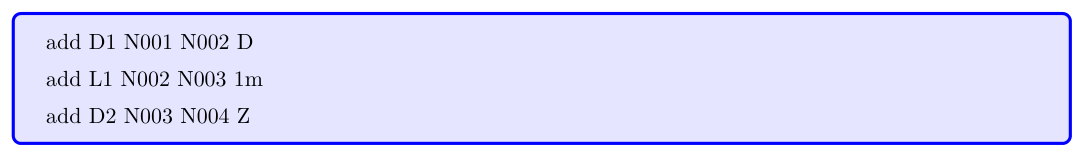
\includegraphics[width=\linewidth,height=.72\textheight,keepaspectratio]{assets/003_p029_vector2.png}\caption{Diagram or recorded result: Project storage requirements.}\label{fig:003_p029_vector20}\end{figure}
\begin{figure}[!htbp]\centering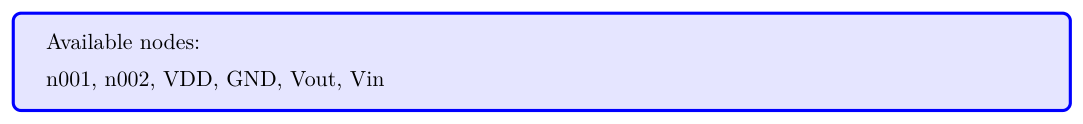
\includegraphics[width=\linewidth,height=.72\textheight,keepaspectratio]{assets/003_p030_vector5.png}\caption{Diagram or recorded result: Project storage requirements.}\label{fig:003_p030_vector50}\end{figure}
\begin{figure}[!htbp]\centering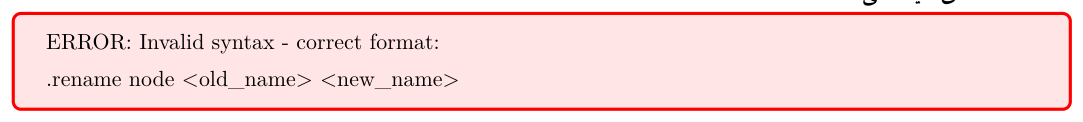
\includegraphics[width=\linewidth,height=.72\textheight,keepaspectratio]{assets/003_p031_vector6.png}\caption{Diagram or recorded result: Project storage requirements.}\label{fig:003_p031_vector60}\end{figure}
\clearpage
\section{Serialization and Cereal}

Serialization converts selected object state into a stored representation, and deserialization reconstructs it. The original JSON example describes two coils, turns, currents, air gap, self/\allowbreak{}mutual inductance, and coupling coefficient. Explicitly list the required fields rather than copying an object's raw in-memory bytes. Pointer values, object padding, virtual-table pointers, and ABI-specific layouts are not portable persistent state. Cereal provides binary, JSON, and XML archives. The assignment chooses binary .bin files and demonstrates installing the header library from its repository. Its sample structure contains src/\allowbreak{}main.cpp, class headers/\allowbreak{}implementations, cereal/\allowbreak{}include, CMakeLists.txt, and a raw.bin result. Add the appropriate include directory to the build. Binary representation can be compact, but it is not encryption and is not guaranteed universally portable across architectures or schema versions. The example Address stores city and ZIP code. Person stores name, age, and a nested Address. Each defines a template serialize(Archive\& ar) method listing its fields. BinaryOutputArchive writes the Person to an ofstream opened in binary mode;\allowbreak{} BinaryInputArchive reconstructs another Person from an ifstream. Check stream and archive errors rather than assuming that every file exists and is valid. The xxd -b raw.bin example demonstrates stored bytes, including string content and numeric fields. Cereal archives the listed fields using their serialization support;\allowbreak{} it does not generally serialize arbitrary complex objects merely by casting their addresses to char* or void*. Likewise, C+\allowbreak{}+\allowbreak{} auto performs compile-time type deduction, rather than runtime evaluation of variable types. Polymorphic component storage requires registration of derived types and relationships. The source illustrates CEREAL\_\allowbreak{}REGISTER\_\allowbreak{}TYPE for Circle and Rectangle and CEREAL\_\allowbreak{}REGISTER\_\allowbreak{}POLYMORPHIC\_\allowbreak{}RELATION with Shape. Apply the corresponding pattern to the Element hierarchy and include the appropriate archive/\allowbreak{}type support. Saving through a base-class pointer without this support can fail or lose the derived representation. Preserve object identity and endpoint references when reconstructing the circuit.

\begin{figure}[!htbp]\centering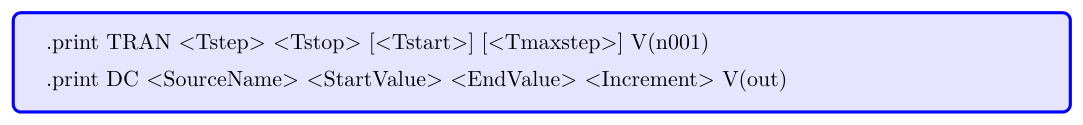
\includegraphics[width=\linewidth,height=.72\textheight,keepaspectratio]{assets/003_p032_vector2.png}\caption{Diagram or recorded result: Serialization and Cereal.}\label{fig:003_p032_vector20}\end{figure}
\begin{figure}[!htbp]\centering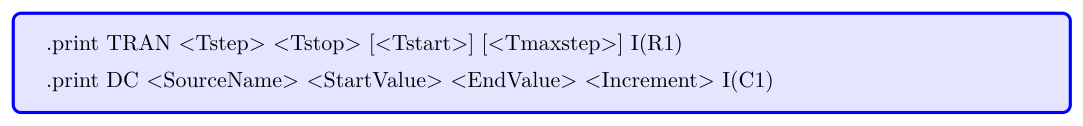
\includegraphics[width=\linewidth,height=.72\textheight,keepaspectratio]{assets/003_p032_vector3.png}\caption{Diagram or recorded result: Serialization and Cereal.}\label{fig:003_p032_vector30}\end{figure}
\begin{figure}[!htbp]\centering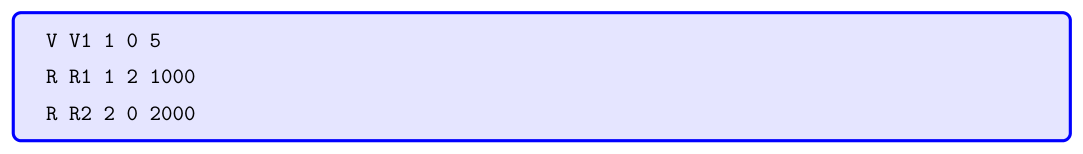
\includegraphics[width=\linewidth,height=.72\textheight,keepaspectratio]{assets/003_p033_vector2.png}\caption{Diagram or recorded result: Serialization and Cereal.}\label{fig:003_p033_vector20}\end{figure}
\begin{figure}[!htbp]\centering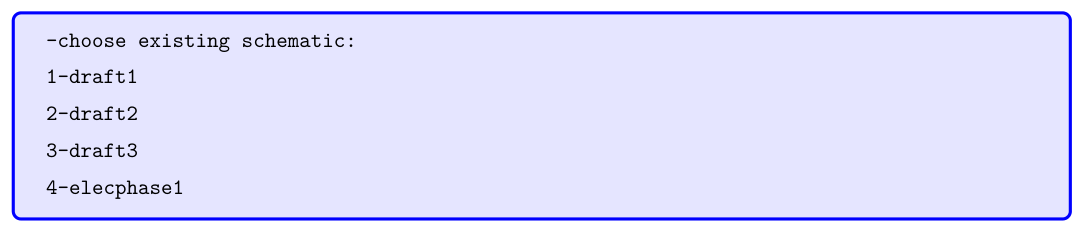
\includegraphics[width=\linewidth,height=.72\textheight,keepaspectratio]{assets/003_p033_vector4.png}\caption{Diagram or recorded result: Serialization and Cereal.}\label{fig:003_p033_vector40}\end{figure}
\begin{figure}[!htbp]\centering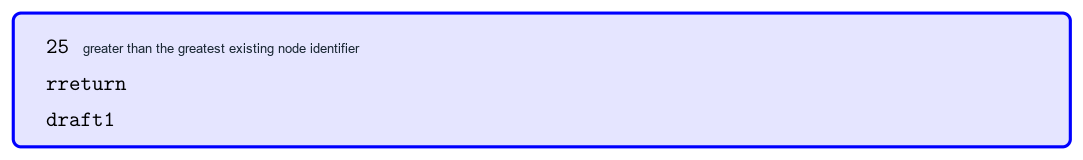
\includegraphics[width=\linewidth,height=.72\textheight,keepaspectratio]{assets/003_p033_vector6.png}\caption{Diagram or recorded result: Serialization and Cereal.}\label{fig:003_p033_vector60}\end{figure}
\begin{figure}[!htbp]\centering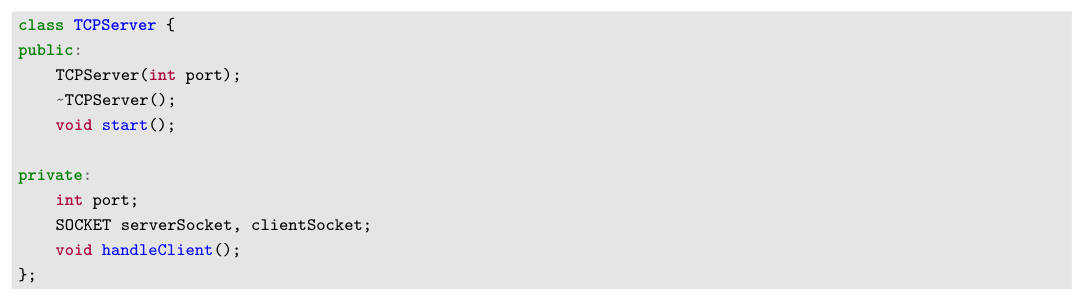
\includegraphics[width=\linewidth,height=.72\textheight,keepaspectratio]{assets/004_p034_vector2.png}\caption{Implementation and output: Serialization and Cereal.}\label{fig:004_p034_vector20}\end{figure}
\begin{figure}[!htbp]\centering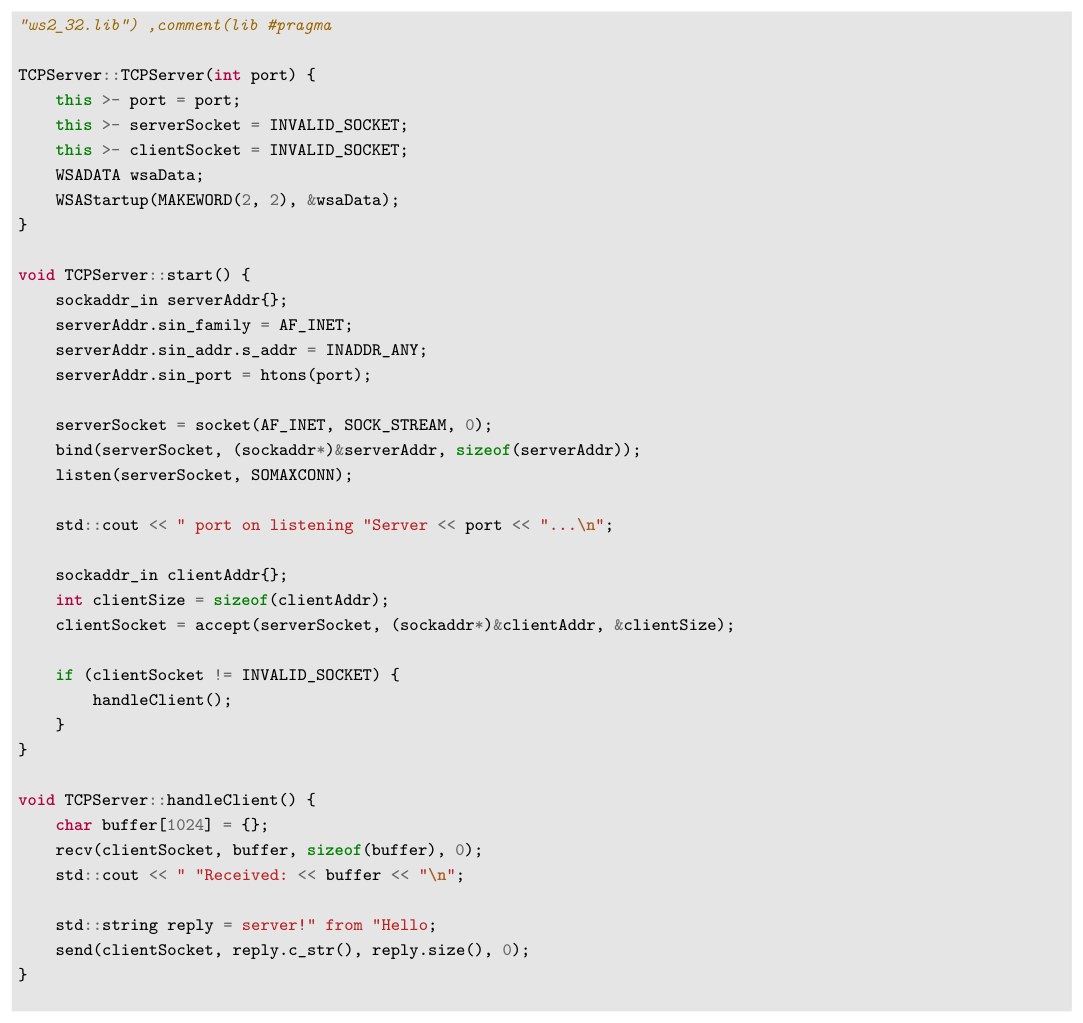
\includegraphics[width=\linewidth,height=.72\textheight,keepaspectratio]{assets/004_p035_vector1.png}\caption{Diagram or recorded result: Serialization and Cereal.}\label{fig:004_p035_vector10}\end{figure}
\clearpage
\section{Networking extension and its limits}

The networking section is bonus work for two-person teams and required for three-person teams under the assignment. Use a server/\allowbreak{}client architecture to transfer an externally generated voltage waveform between two instances. The prescribed demonstration handles one connection at a time;\allowbreak{} concurrent multi-client service is not required. The server listens, accepts a connection, exchanges data, and closes it. The client connects, exchanges data, and closes it. IPv4 addresses are 32 bits (four bytes). IPv6 addresses are 128 bits (sixteen bytes). DNS maps domain names to address records. Ports identify transport endpoints associated with processes/\allowbreak{}services. A socket provides the operating-system interface for connection and data exchange;\allowbreak{} the protocol and application framing remain separate responsibilities. The source's Windows example uses winsock2.h, WSAStartup, AF\_\allowbreak{}INET/\allowbreak{}SOCK\_\allowbreak{}STREAM, bind, listen, accept, recv, send, closesocket, and the ws2\_\allowbreak{}32 library. TCPServer stores its port and listening/\allowbreak{}connected socket handles. TCPClient stores the server address and port. A reusable implementation must check return values, close handles, perform WSACleanup appropriately, and handle partial send/\allowbreak{}recv operations. TCP is a byte stream:\allowbreak{} one send does not guarantee one complete matching recv. Serialize a Signal for transfer. A two-second trace at 1000 samples per second contains 2000 samples. At four bytes per float, its sample payload is 8000 bytes, excluding metadata and framing. A single 1024-byte buffer cannot receive that entire payload in one call. Define a length-prefixed message or another explicit frame format and receive until complete. Streaming chunks reduces latency and memory compared with transferring a whole long trace before playback. For the local demonstration, both computers connect to the same LAN. On Windows, ipconfig exposes the server's IPv4 interface address;\allowbreak{} supply that address and the chosen port to the client. A router's gateway address is not the server's address. Private IPv4 addresses are not restricted to 192.168.x.x;\allowbreak{} other private ranges exist. The original university address and nslookup example are historical illustrations, not verified current service endpoints. First demonstrate a transferred voltage source. The further extension transfers a serialized linear resistive subcircuit or its Thevenin/\allowbreak{}Norton equivalent, reconstructs it at the server, and connects it into the server circuit. The assignment limits this equivalent-circuit task to resistive circuits. Sending a full arbitrary dynamic circuit requires additional state and model semantics beyond this example.

\begin{figure}[!htbp]\centering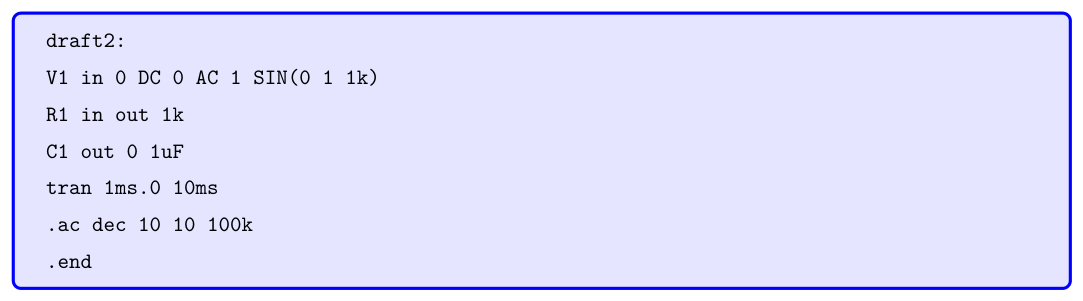
\includegraphics[width=\linewidth,height=.72\textheight,keepaspectratio]{assets/003_p034_vector2.png}\caption{Diagram or recorded result: Networking extension and its limits.}\label{fig:003_p034_vector20}\end{figure}
\begin{figure}[!htbp]\centering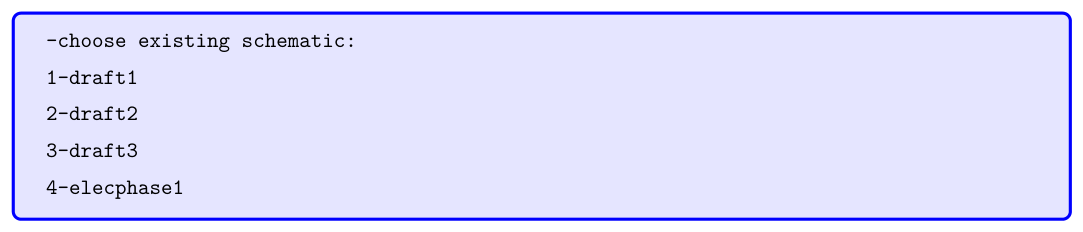
\includegraphics[width=\linewidth,height=.72\textheight,keepaspectratio]{assets/003_p034_vector3.png}\caption{Diagram or recorded result: Networking extension and its limits.}\label{fig:003_p034_vector30}\end{figure}
\begin{figure}[!htbp]\centering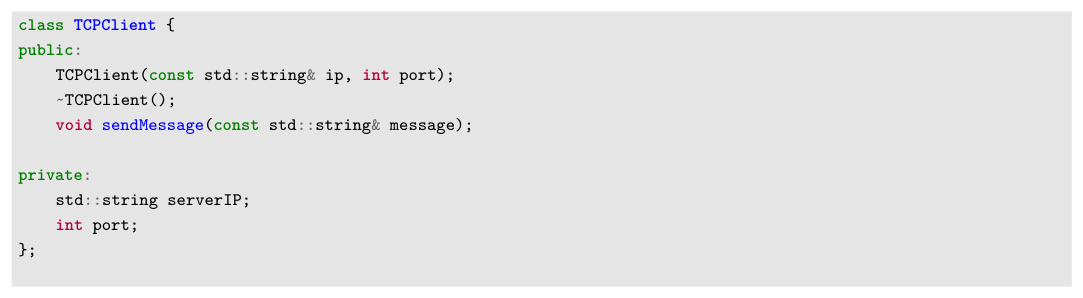
\includegraphics[width=\linewidth,height=.72\textheight,keepaspectratio]{assets/004_p036_vector1.png}\caption{Implementation and output: Networking extension and its limits.}\label{fig:004_p036_vector10}\end{figure}
\begin{figure}[!htbp]\centering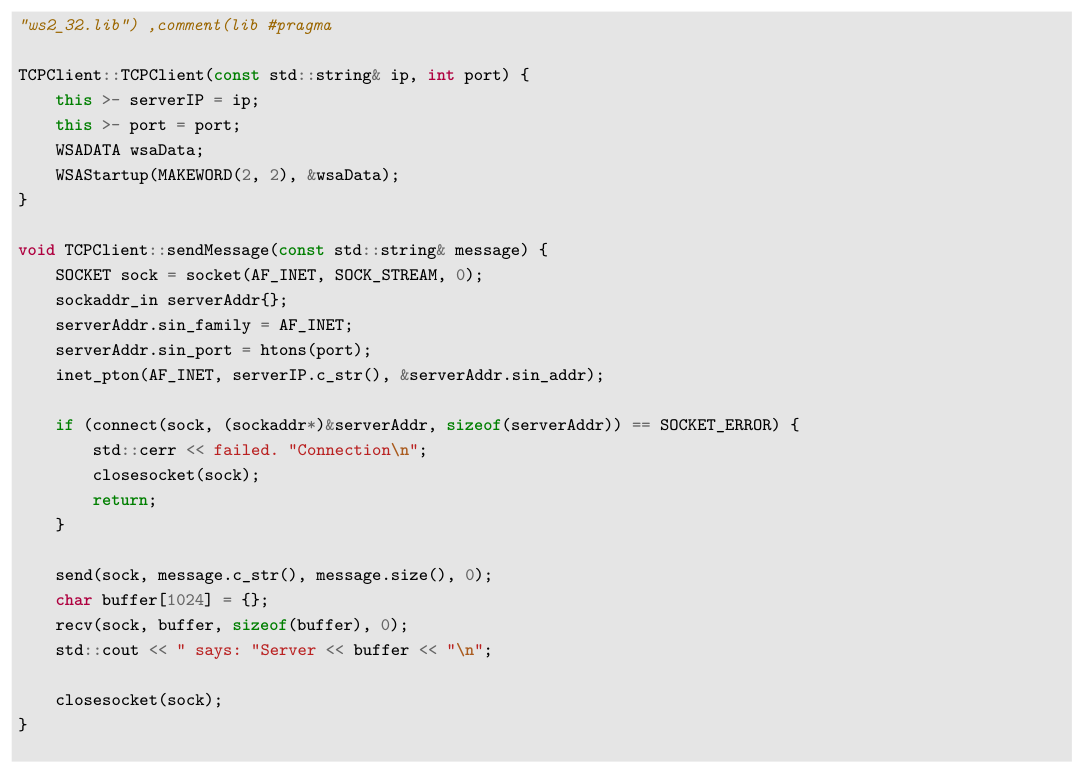
\includegraphics[width=\linewidth,height=.72\textheight,keepaspectratio]{assets/004_p036_vector2.png}\caption{Diagram or recorded result: Networking extension and its limits.}\label{fig:004_p036_vector20}\end{figure}
\begin{figure}[!htbp]\centering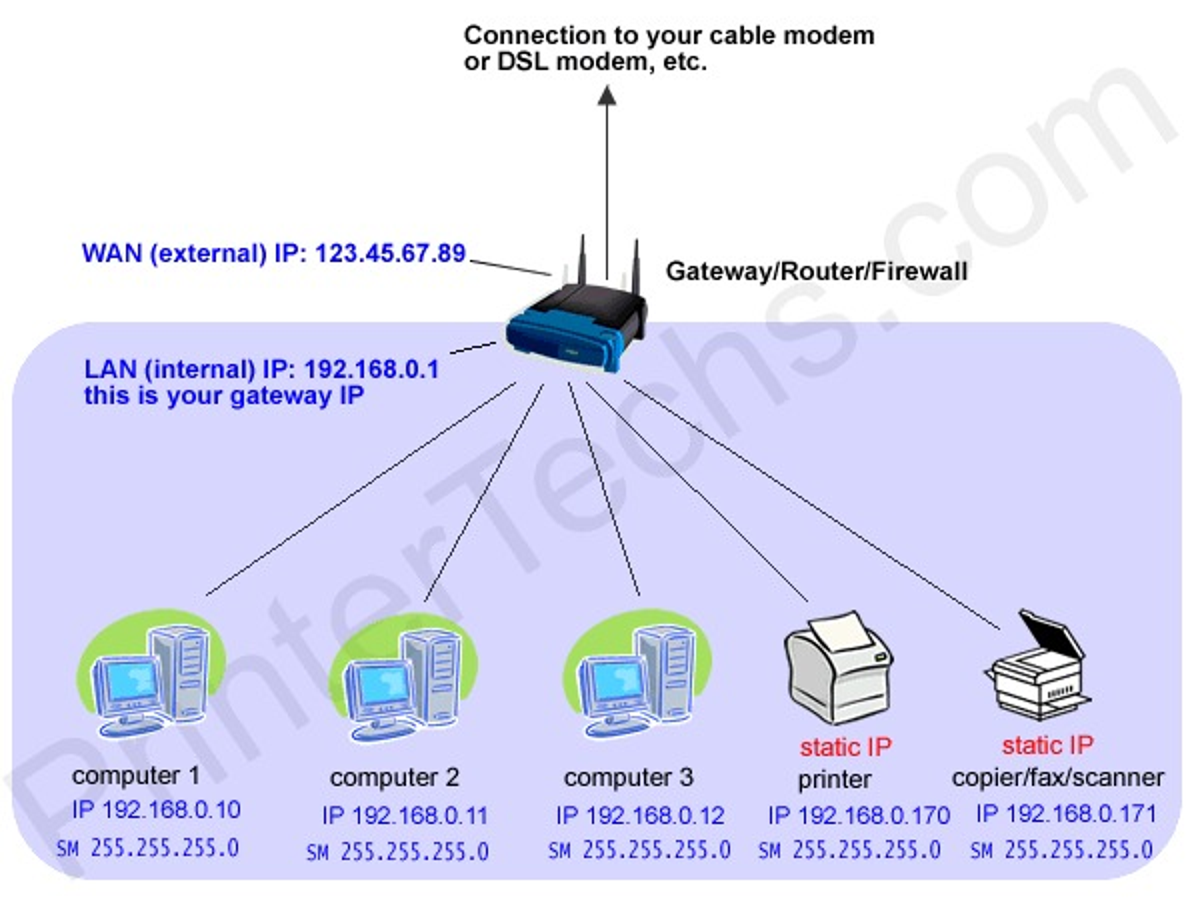
\includegraphics[width=\linewidth,height=.72\textheight,keepaspectratio]{assets/004_p038_01.png}\caption{Diagram or recorded result: Networking extension and its limits.}\label{fig:004_p038_010}\end{figure}
\begin{figure}[!htbp]\centering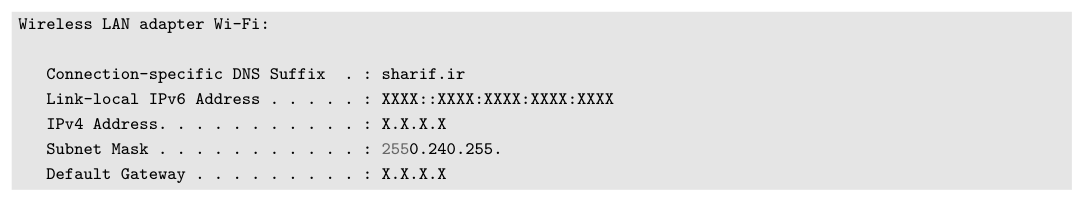
\includegraphics[width=\linewidth,height=.72\textheight,keepaspectratio]{assets/004_p038_vector1.png}\caption{Diagram or recorded result: Networking extension and its limits.}\label{fig:004_p038_vector10}\end{figure}
\clearpage
\section{Deliverable organization}

Submit the graphical source, build configuration, libraries/\allowbreak{}assets required for reproduction, saved-circuit examples, and documented demonstrations. Mark optional and unimplemented features explicitly.

\begin{figure}[!htbp]\centering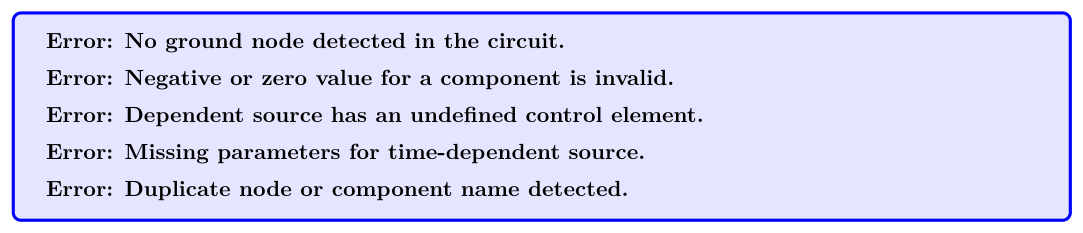
\includegraphics[width=\linewidth,height=.72\textheight,keepaspectratio]{assets/003_p038_vector1.png}\caption{Diagram or recorded result: Deliverable organization.}\label{fig:003_p038_vector10}\end{figure}
\begin{figure}[!htbp]\centering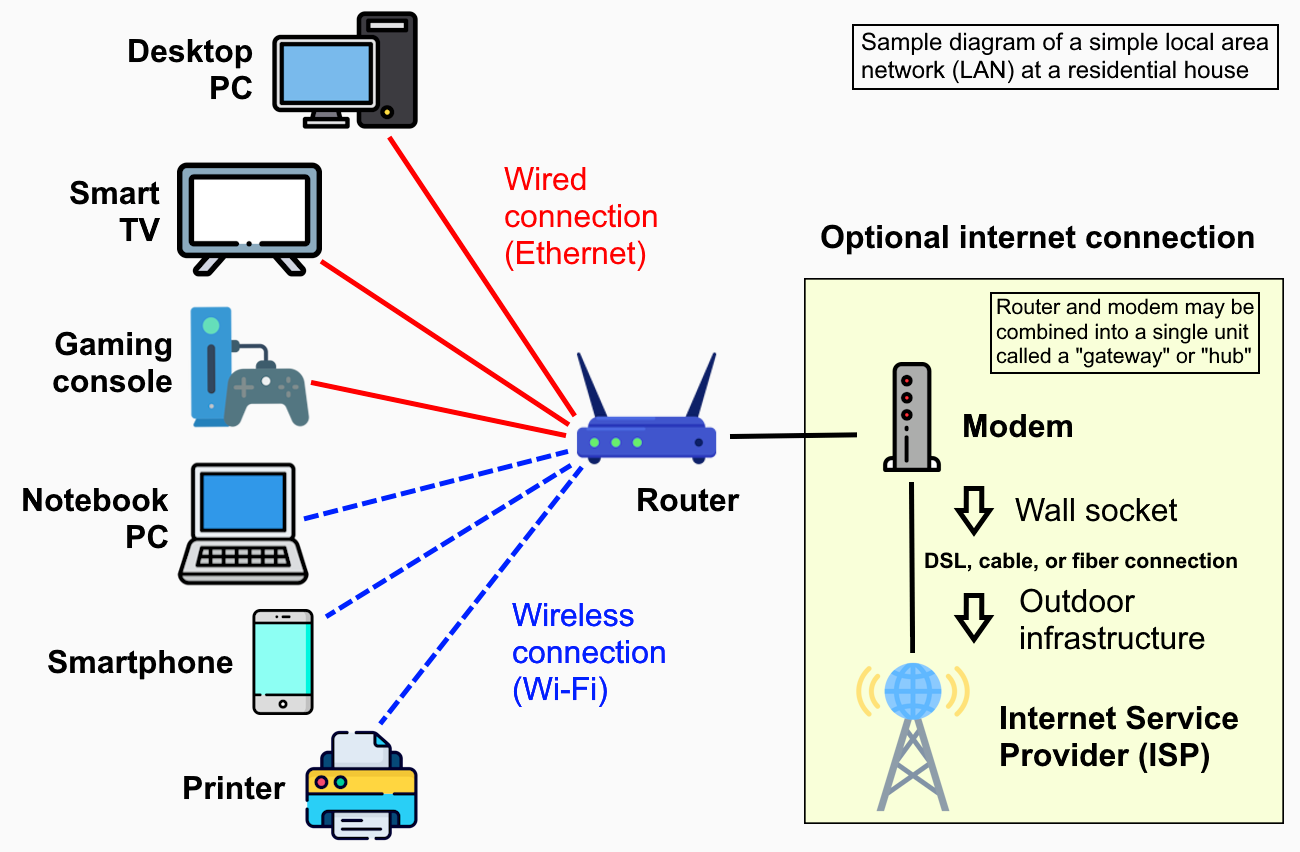
\includegraphics[width=\linewidth,height=.72\textheight,keepaspectratio]{assets/004_p039_01.png}\caption{Diagram or recorded result: Deliverable organization.}\label{fig:004_p039_010}\end{figure}
\begin{figure}[!htbp]\centering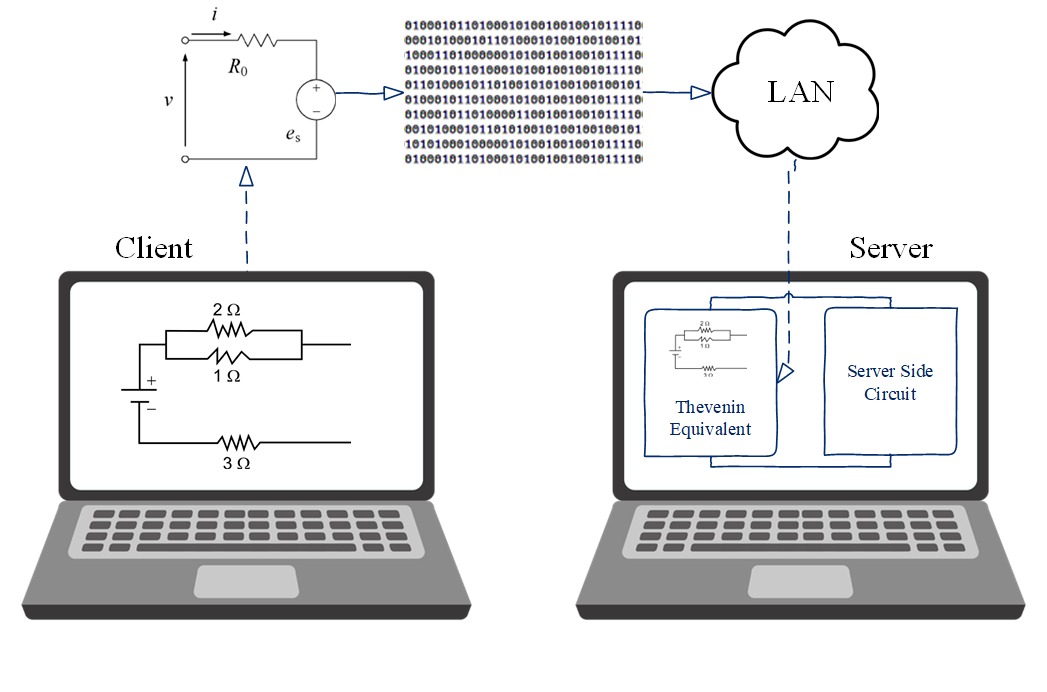
\includegraphics[width=\linewidth,height=.72\textheight,keepaspectratio]{assets/004_p040_01.png}\caption{Diagram or recorded result: Deliverable organization.}\label{fig:004_p040_010}\end{figure}
\clearpage
\end{document}